\section{Languages}
\label{sec:settings-feature-languages}

This page sets the languages the organization uses for its data. Active languages appear in multi-language fields, so a member can write a name in each language, and they are offered as a choice in the organization settings. Adding a language here does not translate the product interface into it. The page opens for anyone with permission to list languages; the add, edit and delete controls appear only for those allowed to use them.

\begin{rcnote}[Example: Horizon]
Horizon works in Arabic and English only, so the system administrator keeps both under “Active” at ②. Horizon does not write its data in Turkish, so the administrator opens that row’s menu at ④, presses “Edit” and sets it to “Inactive”, which moves it to the list at ③.
\end{rcnote}

\begin{figure}[H]
\centering
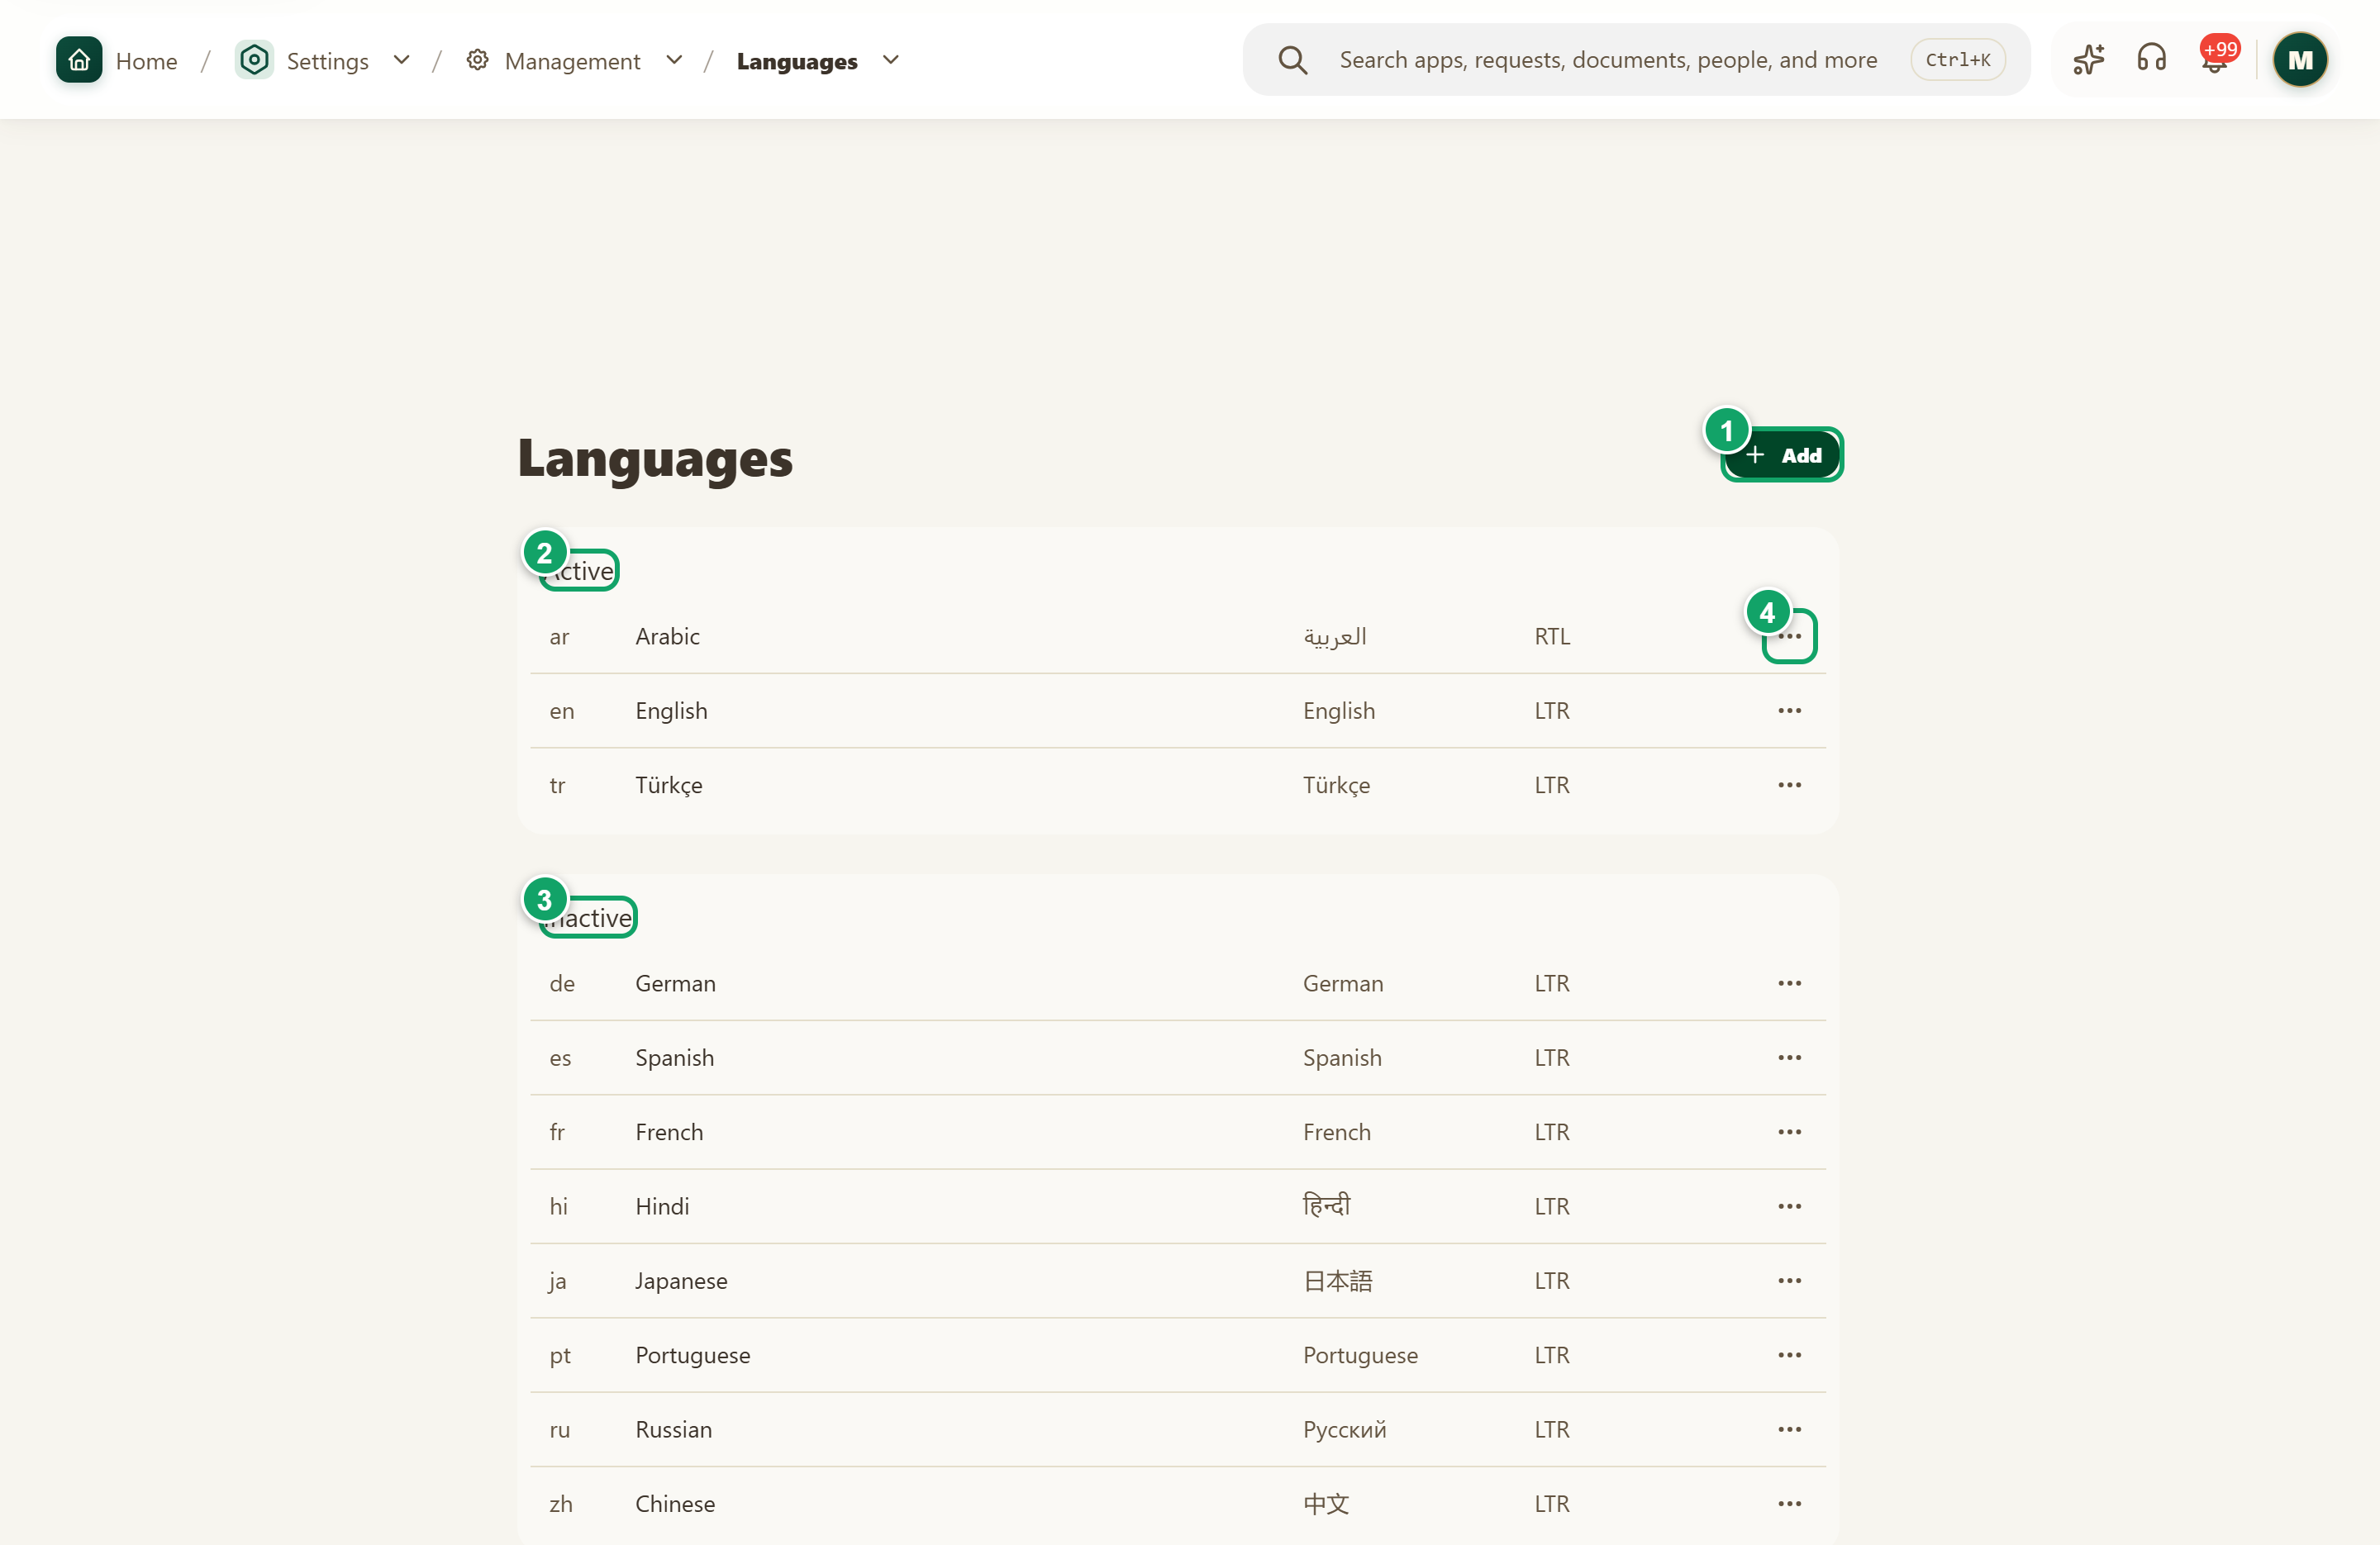
\includegraphics[width=0.95\linewidth,height=0.72\textheight,keepaspectratio]{figures/screens/ch08-languages-en.png}
\caption{Active and inactive languages}
\label{fig:settings-languages-screen}
\shotnote{The page shows the organization’s languages in two lists by status, and each row gives the code, name, native name and writing direction. Moving a language between the lists is safer than deleting it, because its definition stays. ① “Add”. ② “Active”: languages that appear in multi-language fields. ③ “Inactive”: defined languages that are not offered for writing. ④ The three-dot button: opens “Edit” and “Delete”.}
\end{figure}

\begin{figure}[H]
\centering
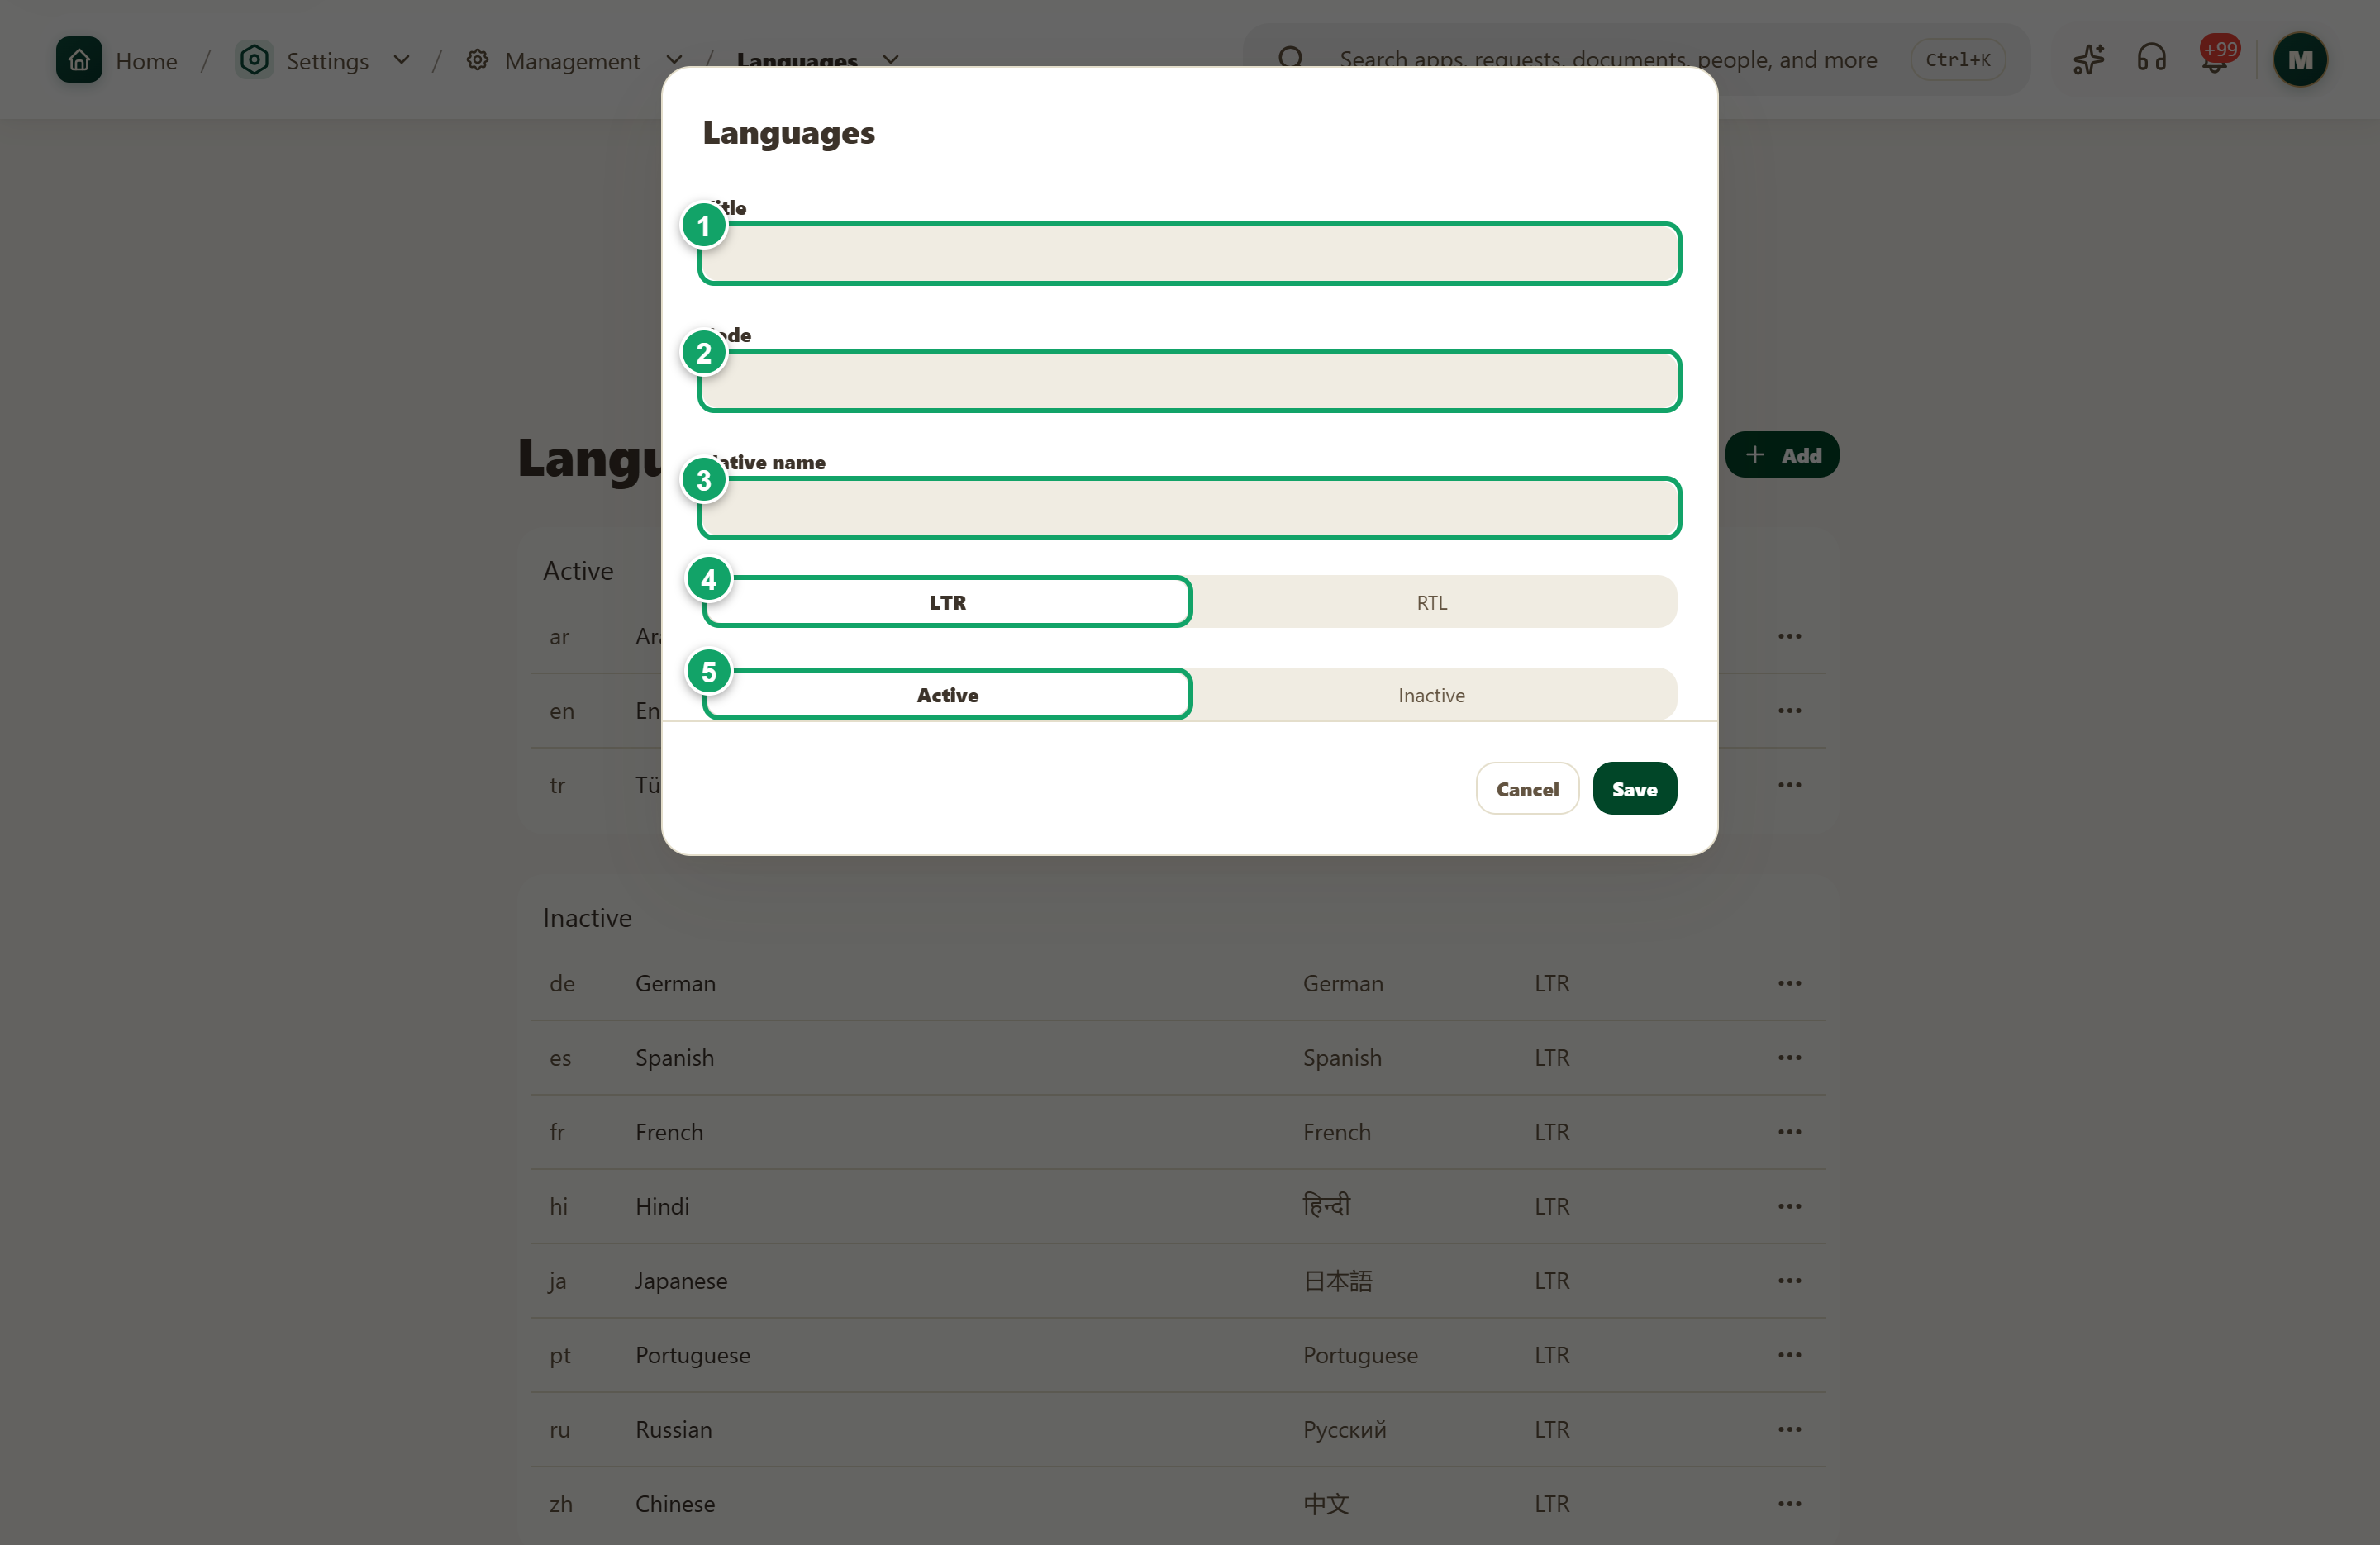
\includegraphics[width=0.95\linewidth,height=0.72\textheight,keepaspectratio]{figures/screens/ch08-languages-form-en.png}
\caption{The add language form}
\label{fig:settings-languages-form-screen}
\shotnote{The window shows the five fields that define a language. It is empty because it was opened to view it and not saved. “Title” and “Code” are enough to save; the other values have a default. ① “Title”. ② “Code”: a short code such as ku; a code already used by another language is refused. ③ “Native name”: the language’s name in its own script. ④ Writing direction. ⑤ Status.}
\end{figure}

\begin{table}[H]
\centering
\caption{What do you record for a language?}
\label{tab:settings-languages-fields}
\begin{tabularx}{\linewidth}{R{4.2cm} Y}
\rcHeaderRow
\thh{Field} & \thh{What to enter}\\
“Title” & The language’s name as you want it shown. Required.\\
“Code” & The language code. Required. Codes that differ only in letter case or spaces count as the same language.\\
“Native name” & The name in its own language, such as «العربية». Optional.\\
Direction & “LTR” or “RTL”.\\
Status & “Active” to offer the language, “Inactive” to keep it defined without offering it.\\
\end{tabularx}
\end{table}

\begin{enumerate}
\item Open “Settings”, then “Languages”.
\item Press “Add”, or open the menu of an existing language and press “Edit”.
\item Enter “Title”, “Code” and “Native name”, then choose the direction and status.
\item Press “Save”. To stop using a language, set it to “Inactive” rather than deleting it.
\end{enumerate}

\textbf{Check:} The language appears in the list that matches its status. Open a multi-language field and confirm that the active language appears there. If the code is refused, the message names the language that already uses it.

\section{Currencies}
\label{sec:settings-feature-currencies}

This page holds what the system needs to work with amounts in more than one currency: the currency list, exchange rates, rate bulletins, rate types, and the rules for rounding and display. The key idea is the “Base currency”, the one currency in which every amount also keeps an equivalent, so that different currencies can be added up in lists and reports. The page opens for anyone with the currencies permission; changing “Money settings” and rate types is limited to the organization owner and holders of the Administrator role.

\begin{rcnote}[Example: Horizon]
Horizon keeps its accounts in Syrian pounds and receives some payments in US dollars. The system administrator makes the pound the base currency, activates the dollar, and presses “Add rate” each morning to record the market rate.
\end{rcnote}

\begin{figure}[H]
\centering
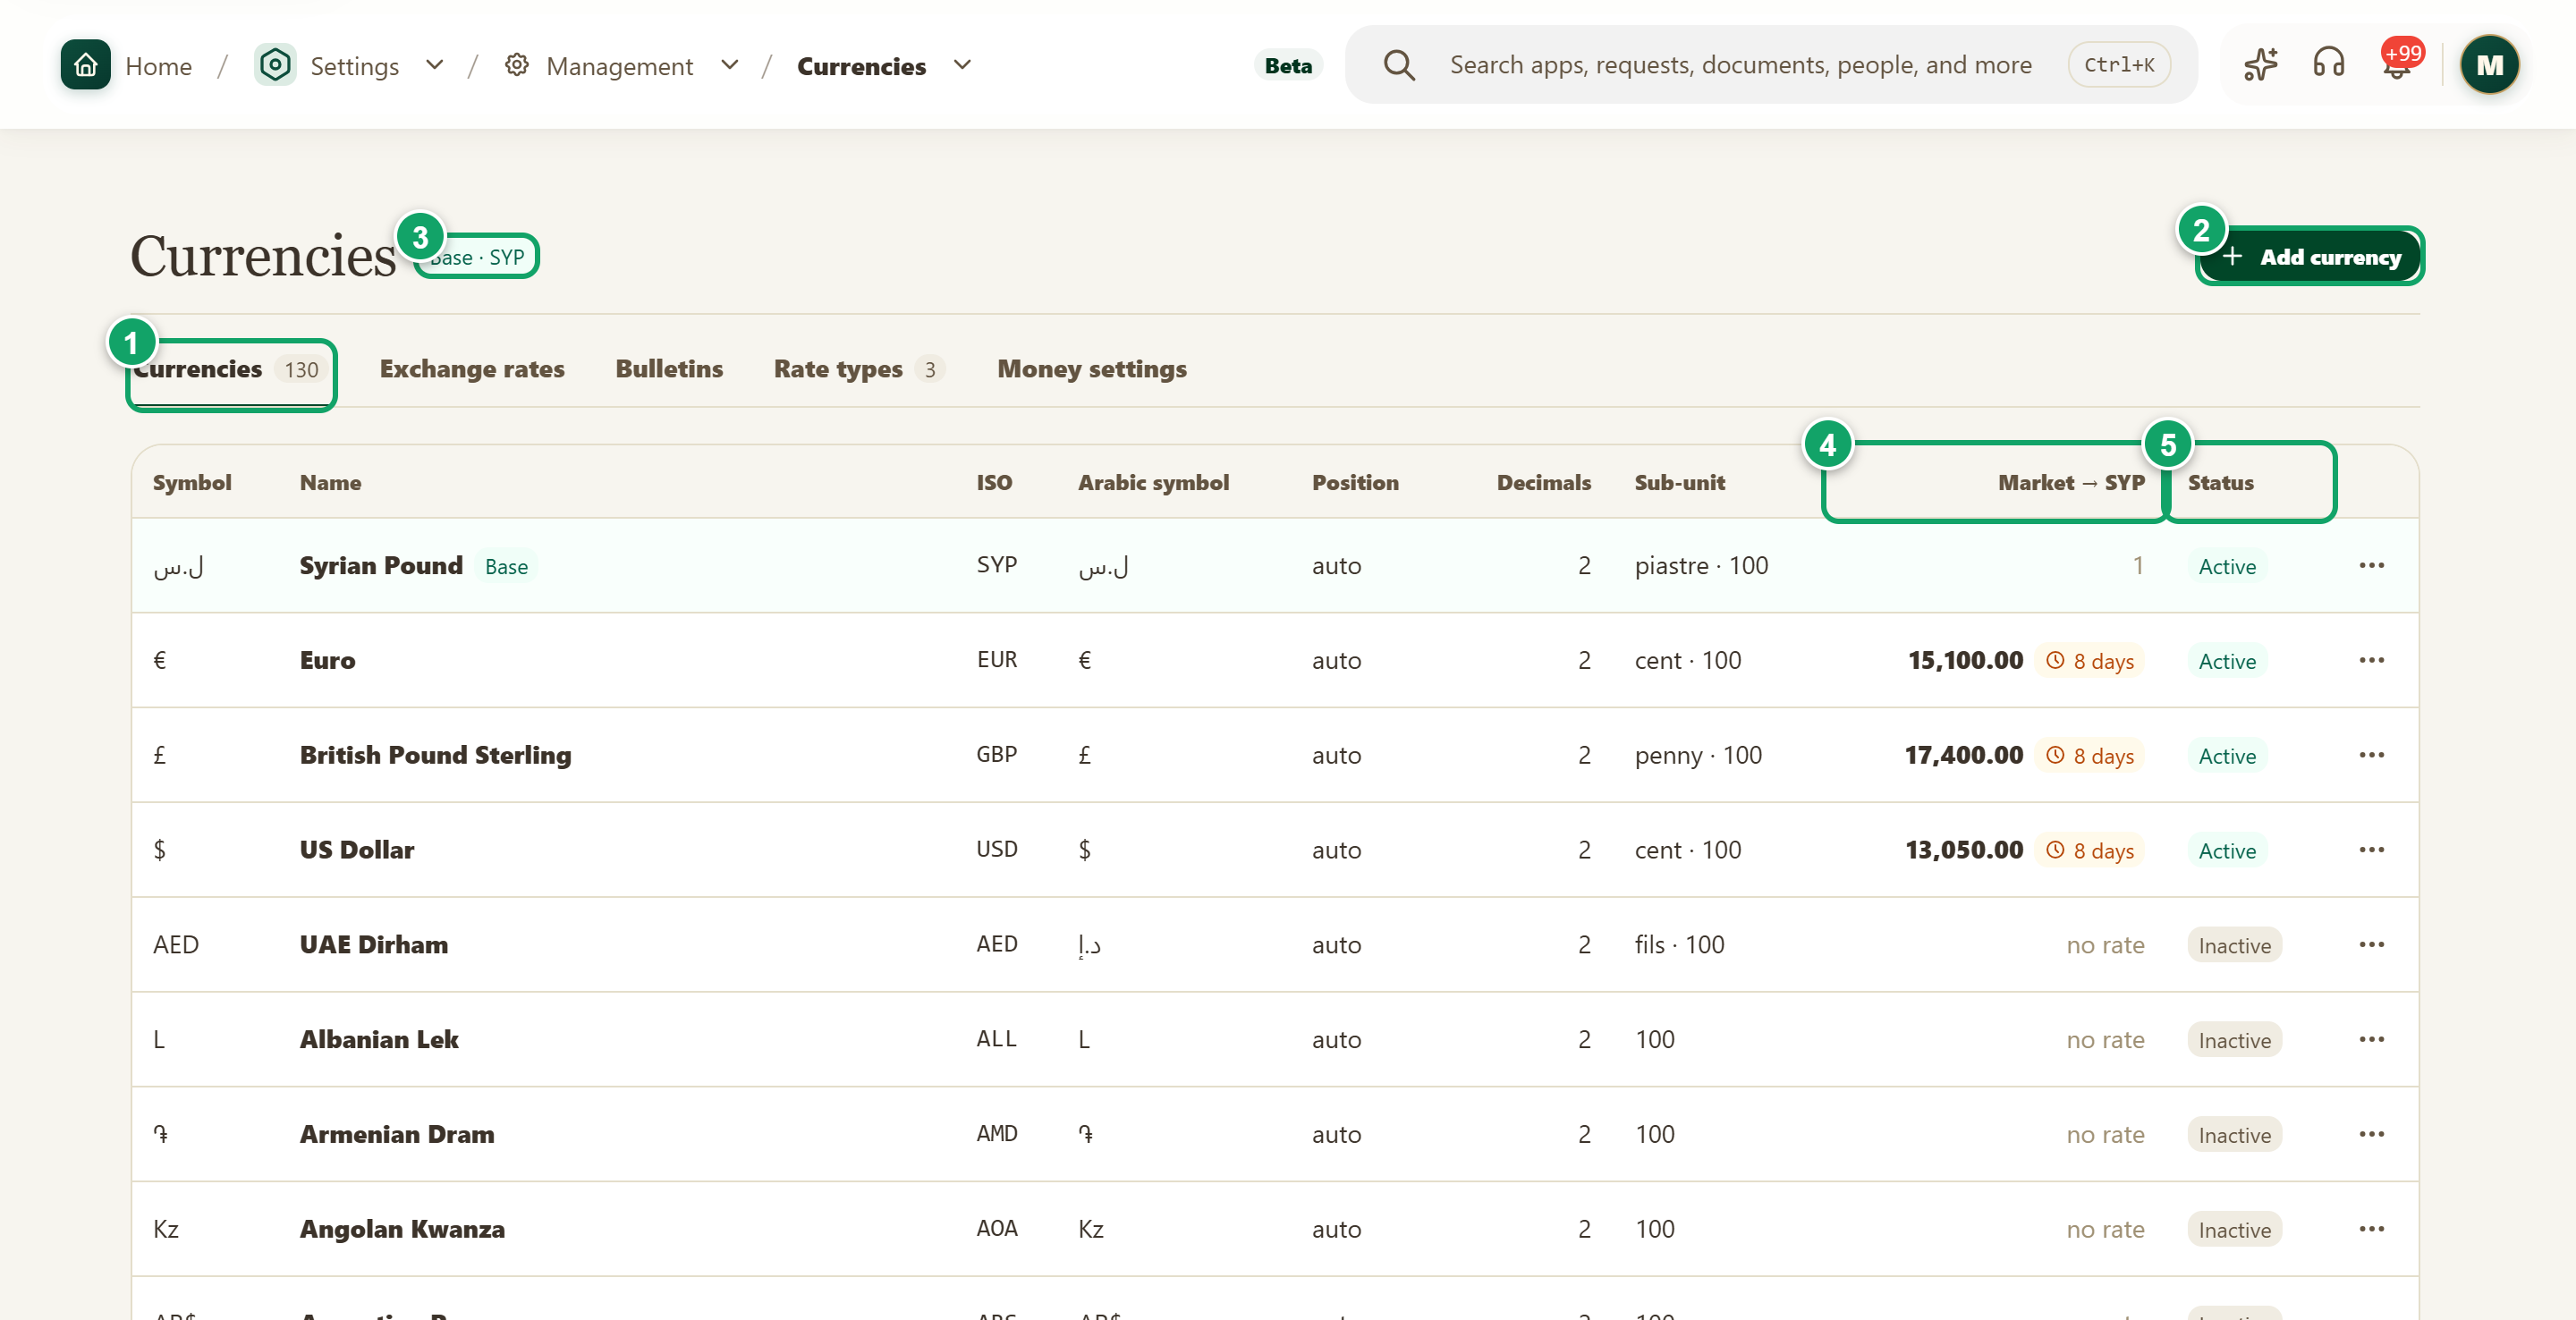
\includegraphics[width=0.95\linewidth,height=0.72\textheight,keepaspectratio]{figures/screens/ch08-currencies-en.png}
\caption{The currency list}
\label{fig:settings-currencies-screen}
\shotnote{The list shows each currency with its symbols, decimals and latest rate against the base currency. Only active currencies can be picked for new values; amounts already saved in an inactive currency stay visible. ① “Currencies”. ② “Add currency”. ③ The “Base” chip: shows the organization’s base currency code. ④ The rate column: the latest rate of the default rate type, with its age when it is getting old. ⑤ “Status”.}
\end{figure}

\begin{table}[H]
\centering
\caption{What do you record for a currency?}
\label{tab:settings-currencies-fields}
\begin{tabularx}{\linewidth}{R{4.2cm} Y}
\rcHeaderRow
\thh{Window tab} & \thh{What you record there}\\
“General” & The three-letter “ISO code”, “Symbol”, “Arabic symbol”, “Name”, “Symbol position”, “Decimal places” and “Status”. The ISO code is fixed once the currency is used, and decimals can only go up while amounts exist.\\
“Units \& words” & “Sub-unit ratio”, such as 100 piastres to the pound, and the unit names used when an amount is written in words.\\
“Denominations” & An old unit of the same currency, as in a redenomination: 100 old = 1 new. Amounts are always stored in the current unit.\\
\end{tabularx}
\end{table}

\begin{figure}[H]
\centering
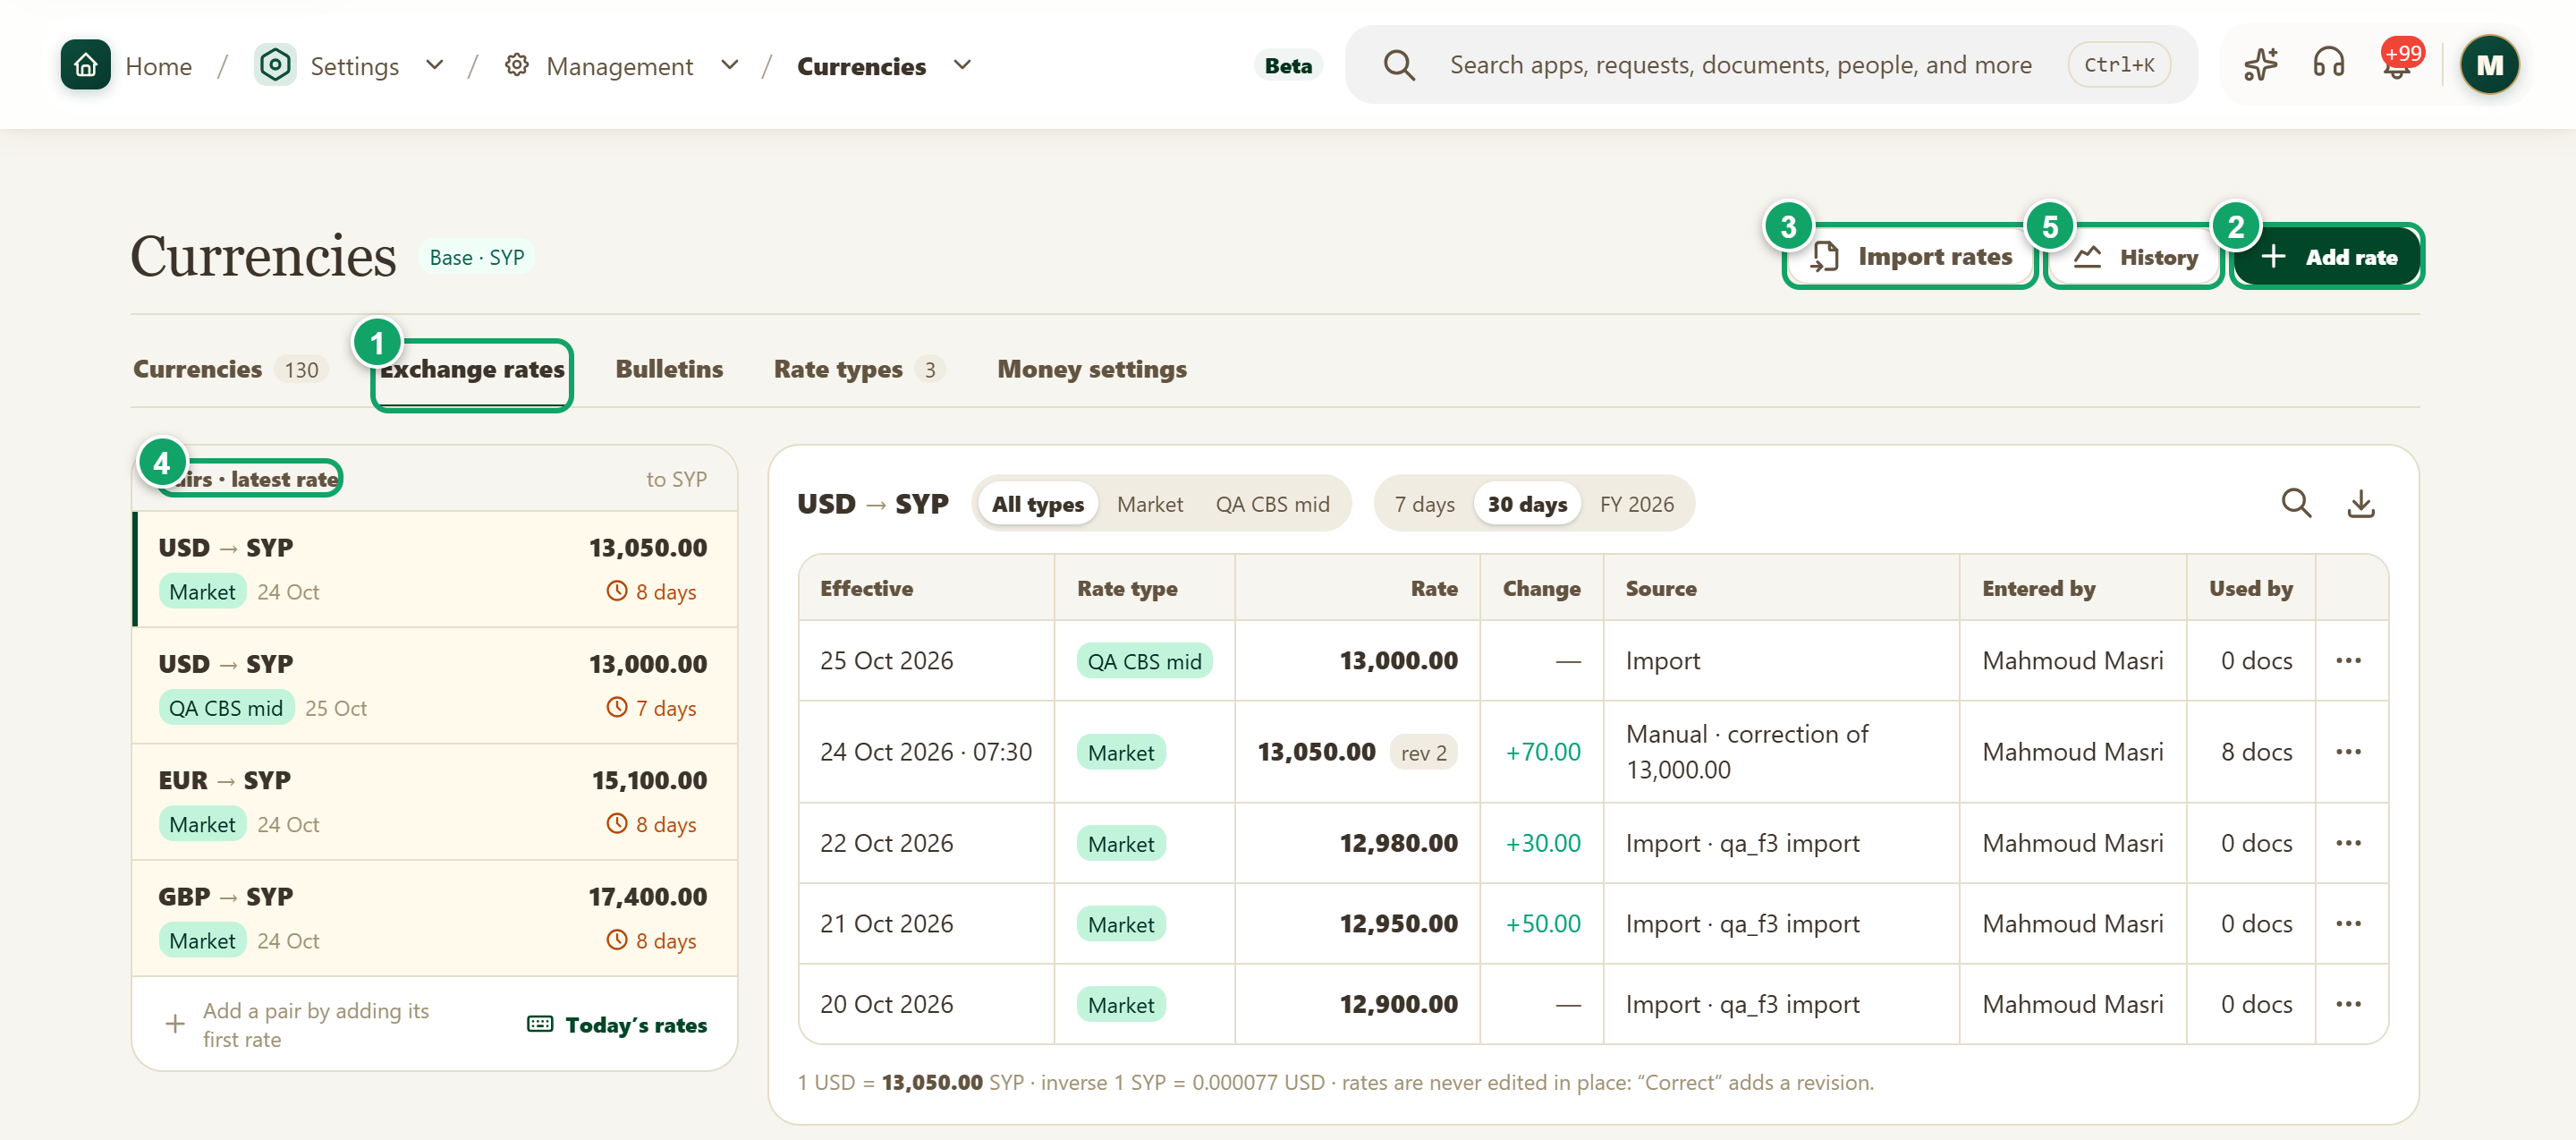
\includegraphics[width=0.95\linewidth,height=0.72\textheight,keepaspectratio]{figures/screens/ch08-currencies-rates-en.png}
\caption{Exchange rates}
\label{fig:settings-currencies-rates-screen}
\shotnote{The tab shows currency pairs with the latest rate of each, and the rate history of the selected pair. Rates are never edited in place: “Correct…” adds a revision and keeps the original, so you can always see who entered a rate and where it came from. ① “Exchange rates”. ② “Add rate”: choose the rate type, currencies and date, and type the rate. ③ “Import rates”: uploads several rates from a file. ④ “Pairs · latest rate”: pick a pair to see its history. ⑤ “History”: shows the rate over time on a chart.}
\end{figure}

\begin{figure}[H]
\centering
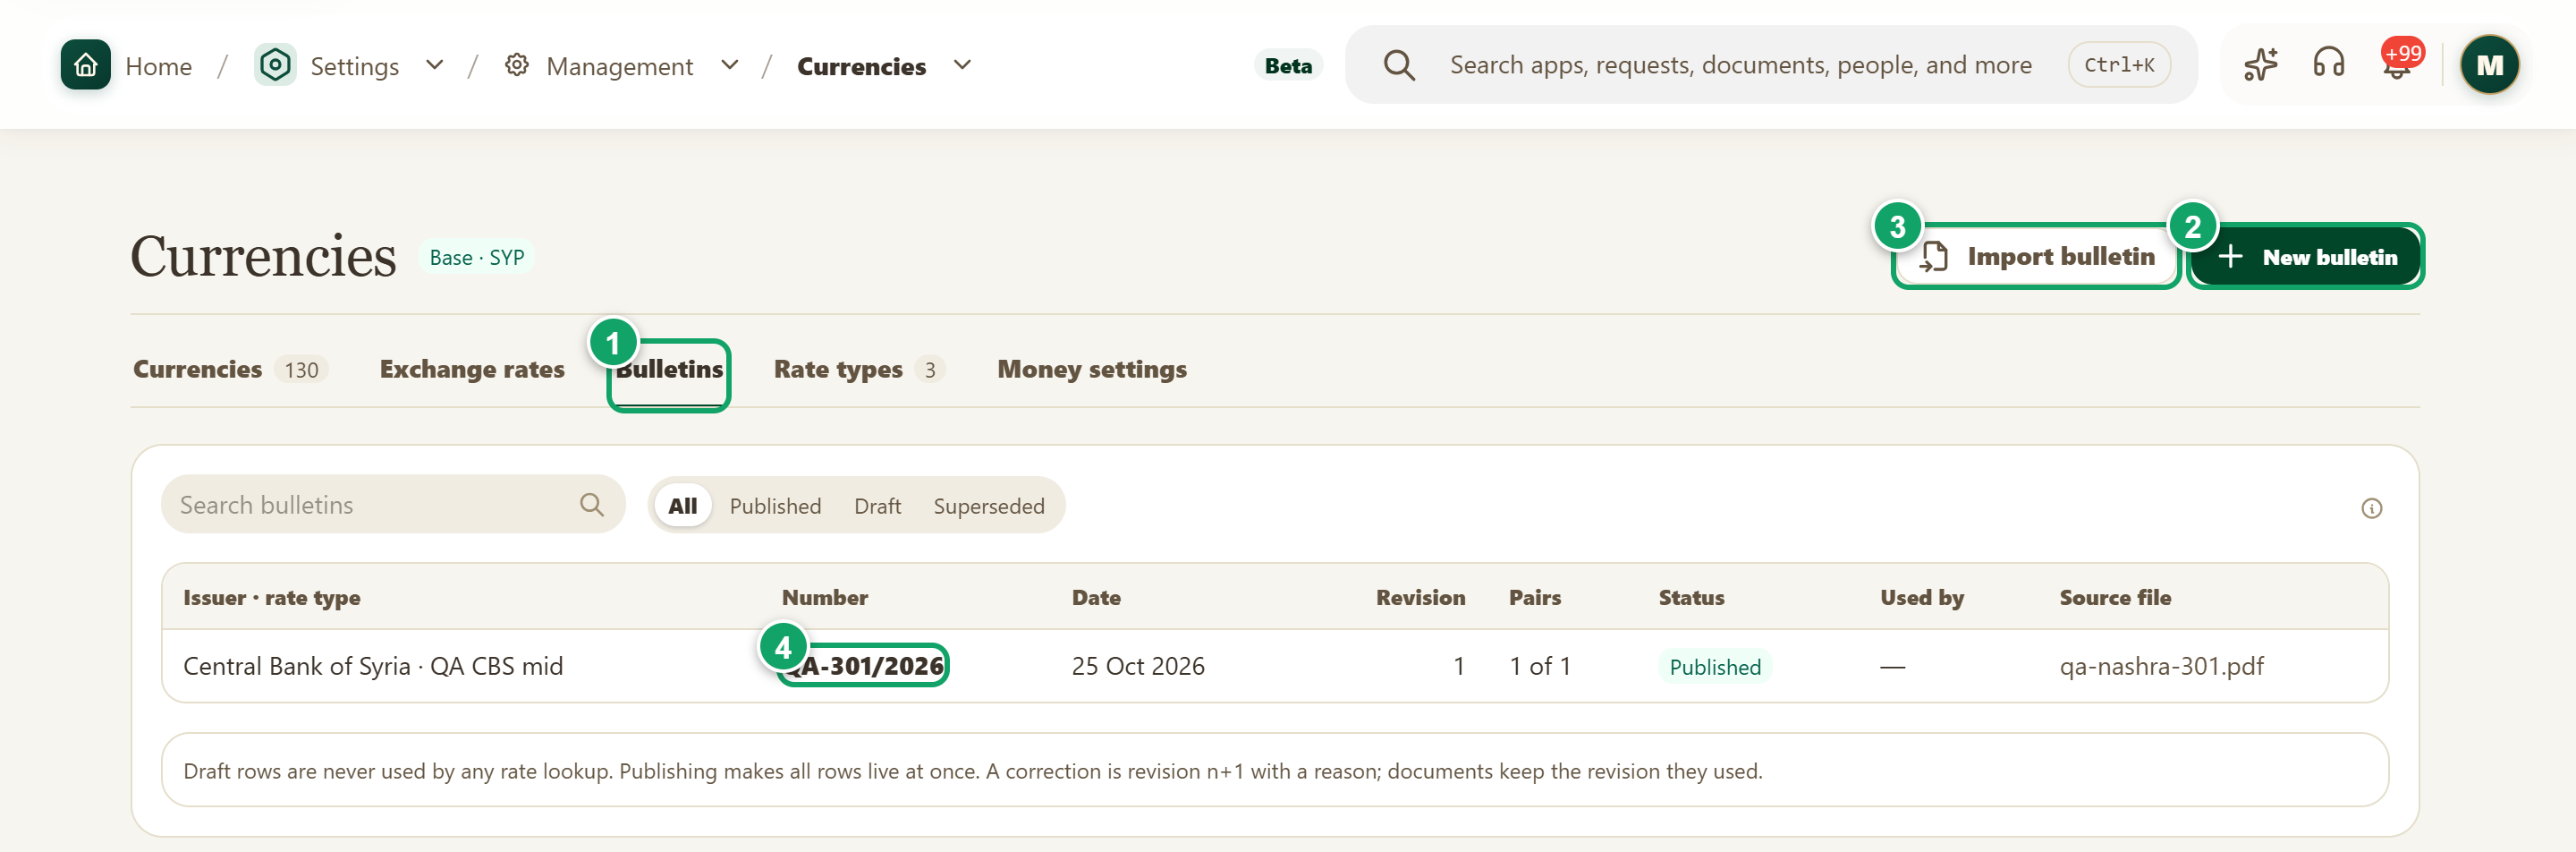
\includegraphics[width=0.95\linewidth,height=0.72\textheight,keepaspectratio]{figures/screens/ch08-currencies-bulletins-en.png}
\caption{Rate bulletins}
\label{fig:settings-currencies-bulletins-screen}
\shotnote{A bulletin is a dated, numbered set of rates from one issuer, such as a central bank. The system ignores its draft. Once published, all its rows become live together, and it changes only through a correction revision with a reason. ① “Bulletins”. ② “New bulletin”. ③ “Import bulletin”. ④ The bulletin number: open it to read its rows.}
\end{figure}

\begin{figure}[H]
\centering
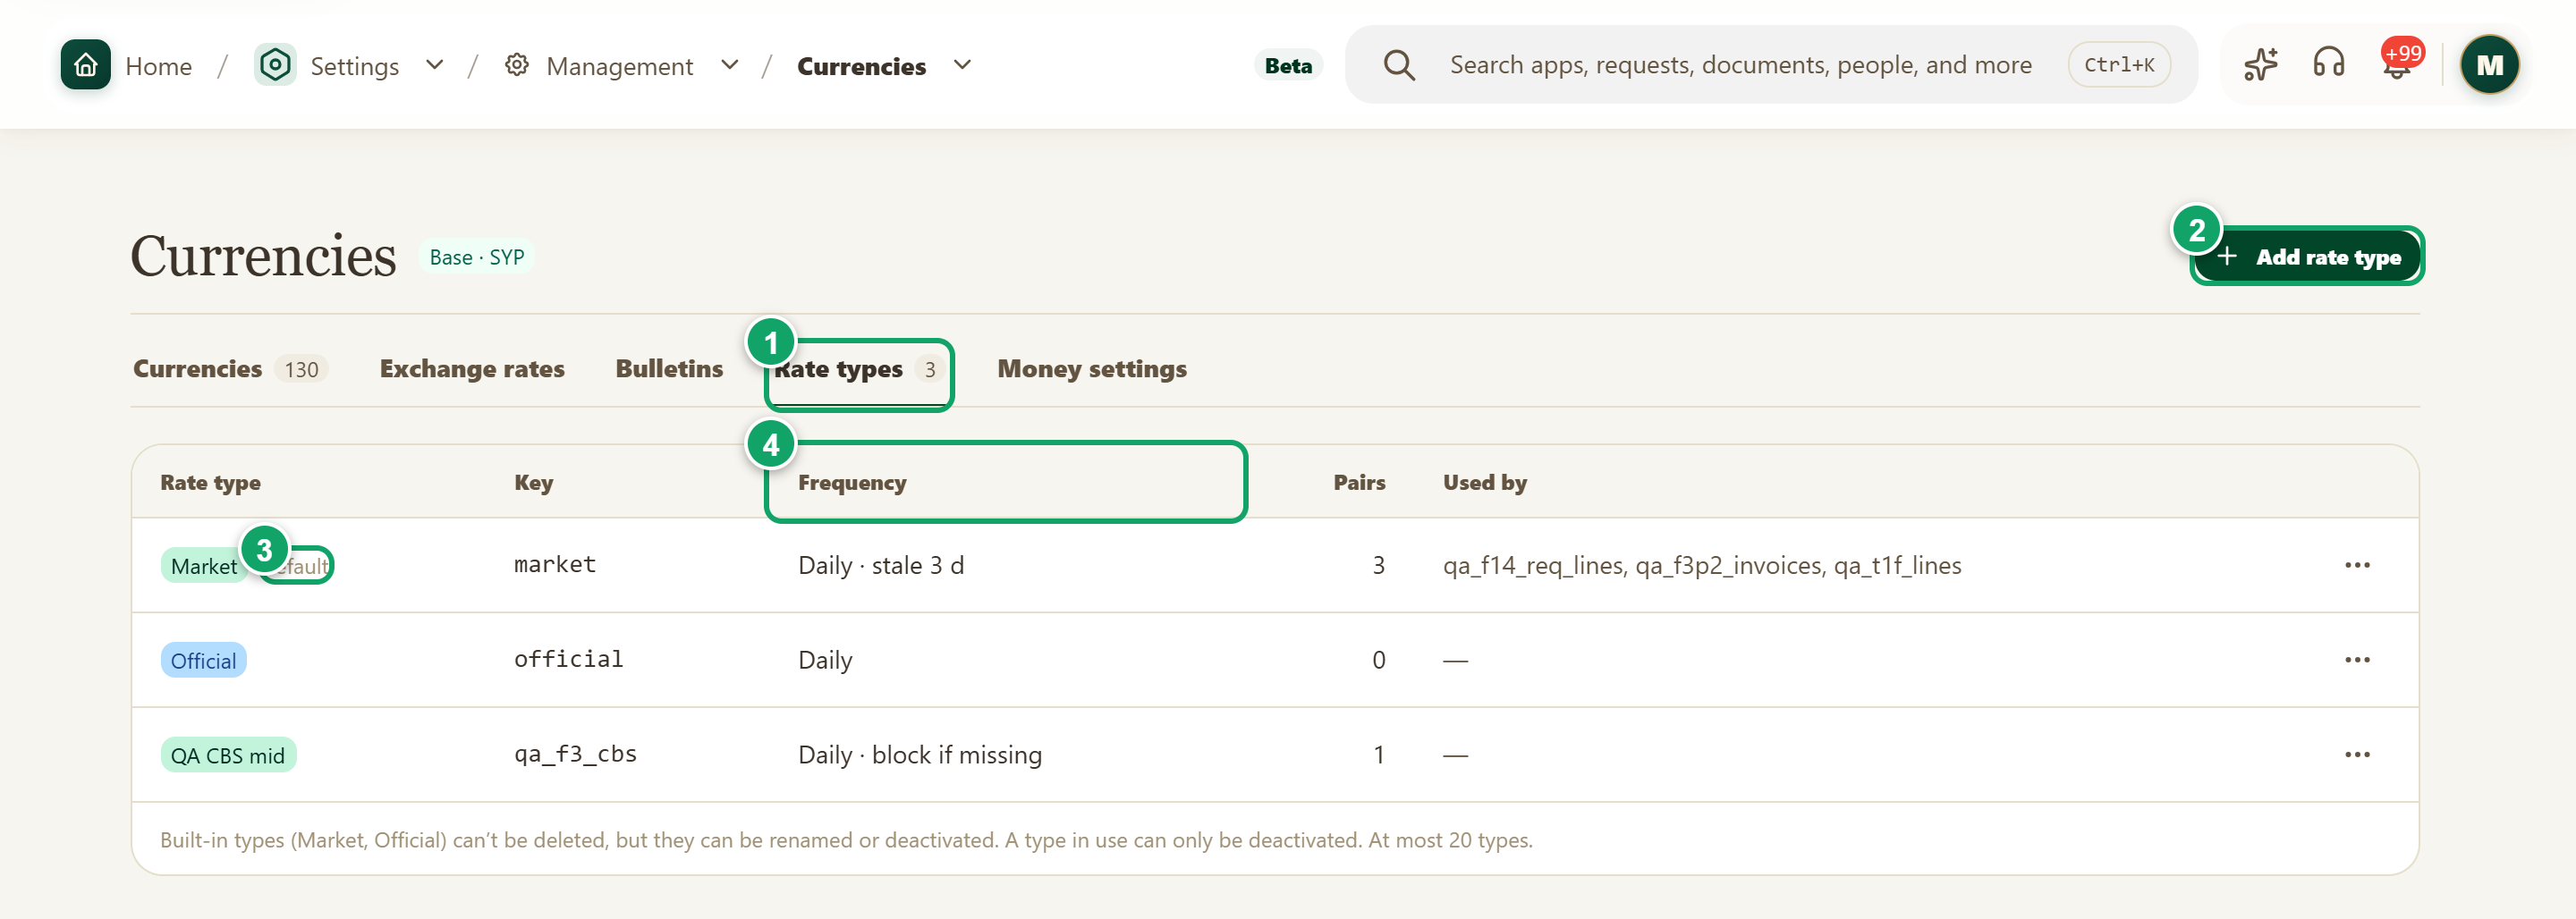
\includegraphics[width=0.95\linewidth,height=0.72\textheight,keepaspectratio]{figures/screens/ch08-currencies-rate-types-en.png}
\caption{Rate types}
\label{fig:settings-currencies-rate-types-screen}
\shotnote{A rate type is a named source of rates, such as the market rate or a bank’s circular. Types help when one currency has more than one rate on the same day. ① “Rate types”. ② “Add rate type”. ③ “default”: the type used when a document does not choose one. ④ “Frequency”: how often an update is expected and when a rate counts as stale.}
\end{figure}

\begin{figure}[H]
\centering
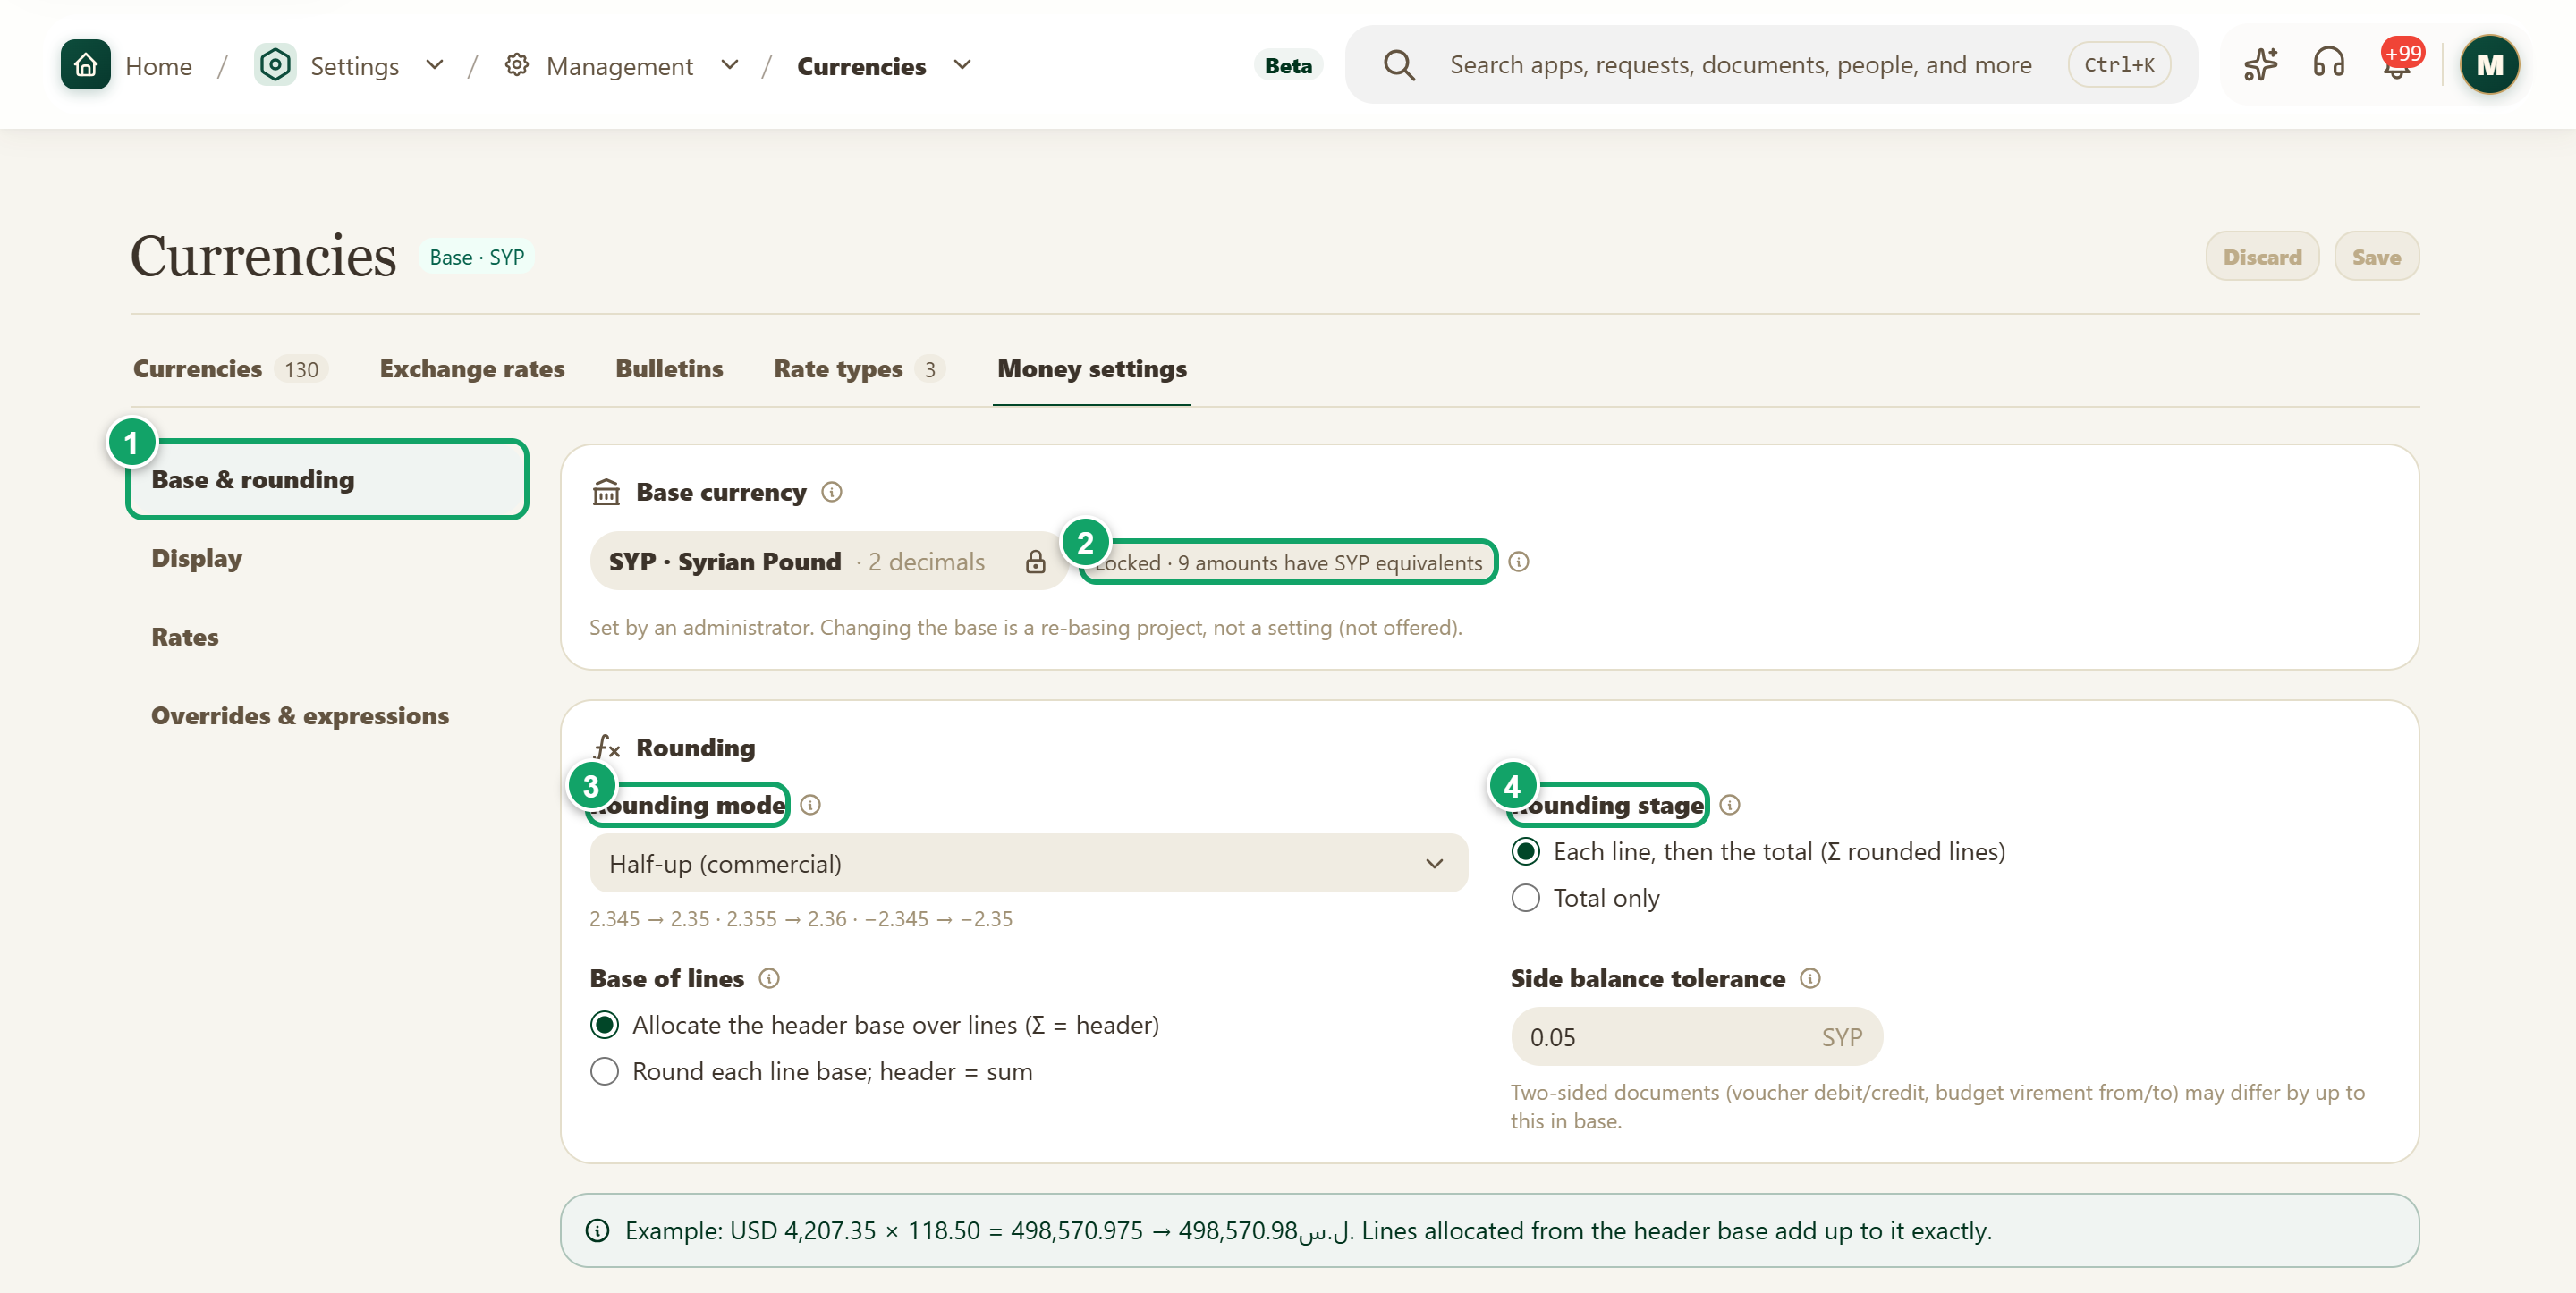
\includegraphics[width=0.95\linewidth,height=0.72\textheight,keepaspectratio]{figures/screens/ch08-currencies-settings-en.png}
\caption{Money settings: base and rounding}
\label{fig:settings-currencies-settings-screen}
\shotnote{This section sets the base currency and how amounts are rounded on every document. The lock is deliberate: after the first document saves an equivalent, changing the base is no longer offered. ① “Base \& rounding”. ② The lock chip: shows how many amounts depend on the base currency. ③ “Rounding mode”. ④ “Rounding stage”: round each line and add them, or round the total only.}
\end{figure}

\begin{figure}[H]
\centering
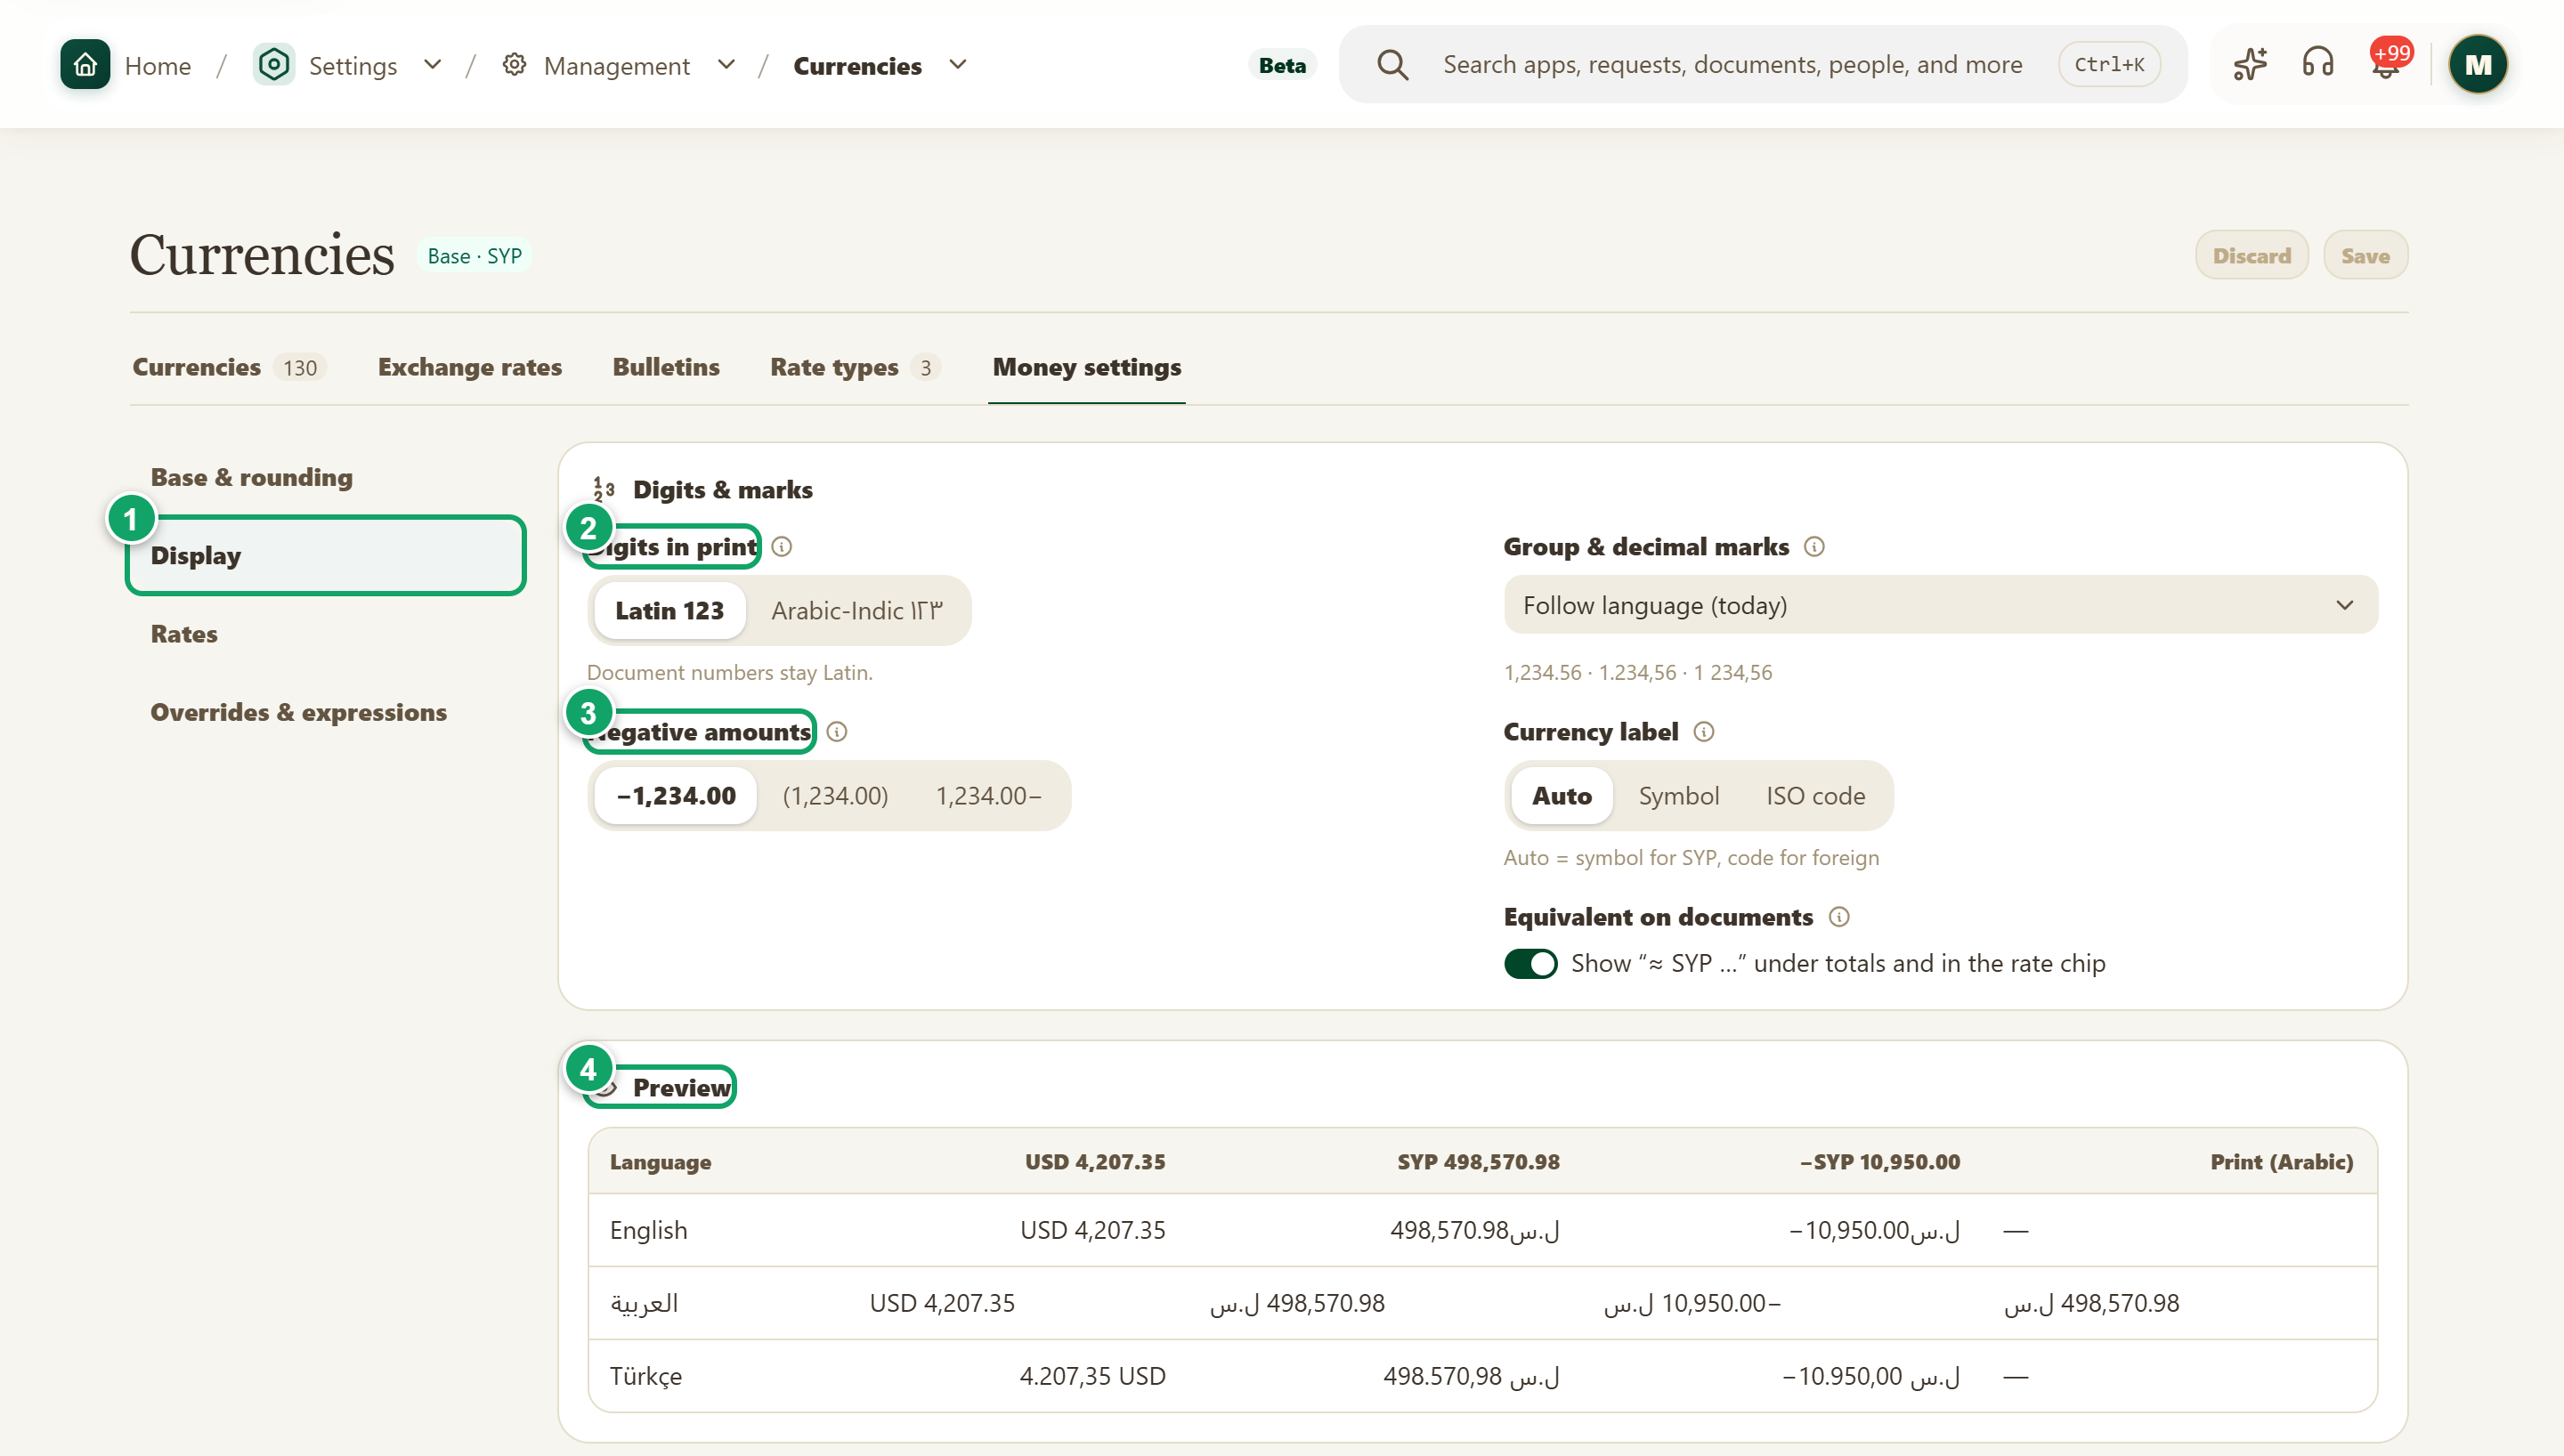
\includegraphics[width=0.95\linewidth,height=0.72\textheight,keepaspectratio]{figures/screens/ch08-currencies-settings-display-en.png}
\caption{Money settings: display}
\label{fig:settings-currencies-settings-display-screen}
\shotnote{This section changes only how amounts read, not their saved values. The preview shows the effect in each active language before you save. ① “Display”. ② “Digits in print”. ③ “Negative amounts”. ④ “Preview”.}
\end{figure}

\begin{figure}[H]
\centering
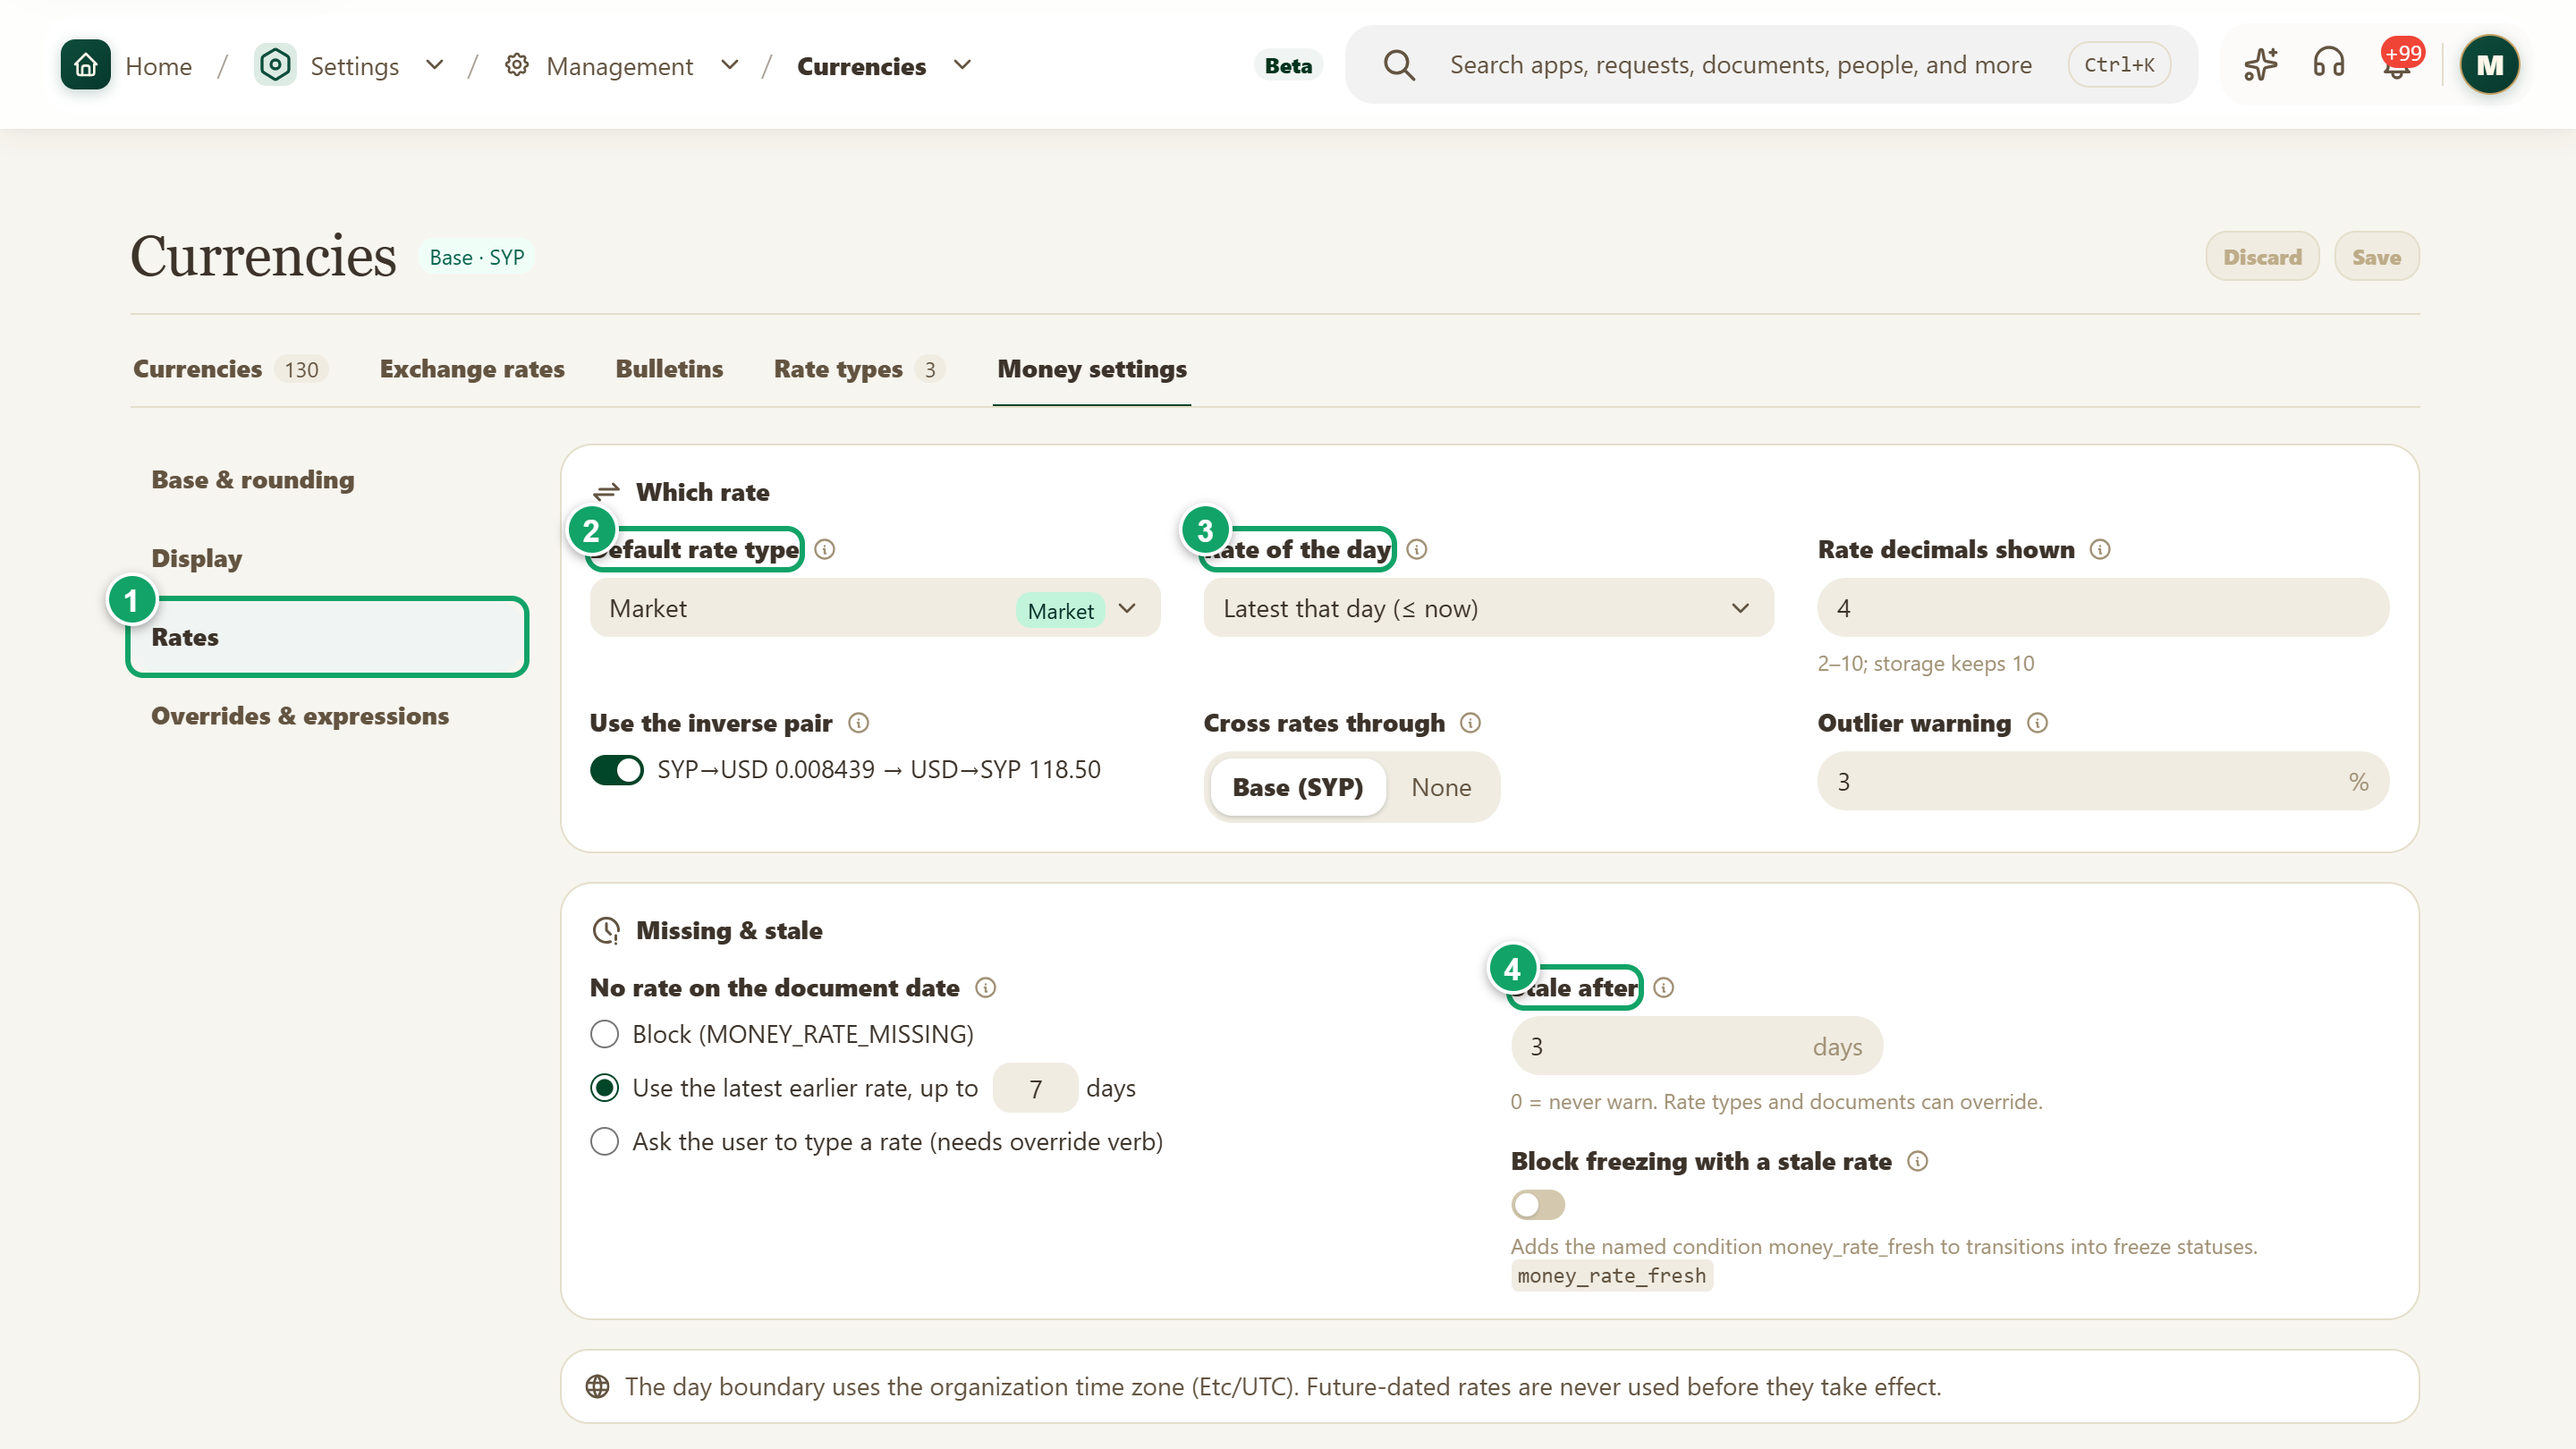
\includegraphics[width=0.95\linewidth,height=0.72\textheight,keepaspectratio]{figures/screens/ch08-currencies-settings-rates-en.png}
\caption{Money settings: rates}
\label{fig:settings-currencies-settings-rates-screen}
\shotnote{This section decides which rate the system picks for a document, and what happens when a rate is missing or old. The start and end of a day use the organization’s time zone, and a rate is never used before its effective date. ① “Rates”. ② “Default rate type”. ③ “Rate of the day”: for days with more than one rate. ④ “Stale after”: zero means no warning.}
\end{figure}

\begin{figure}[H]
\centering
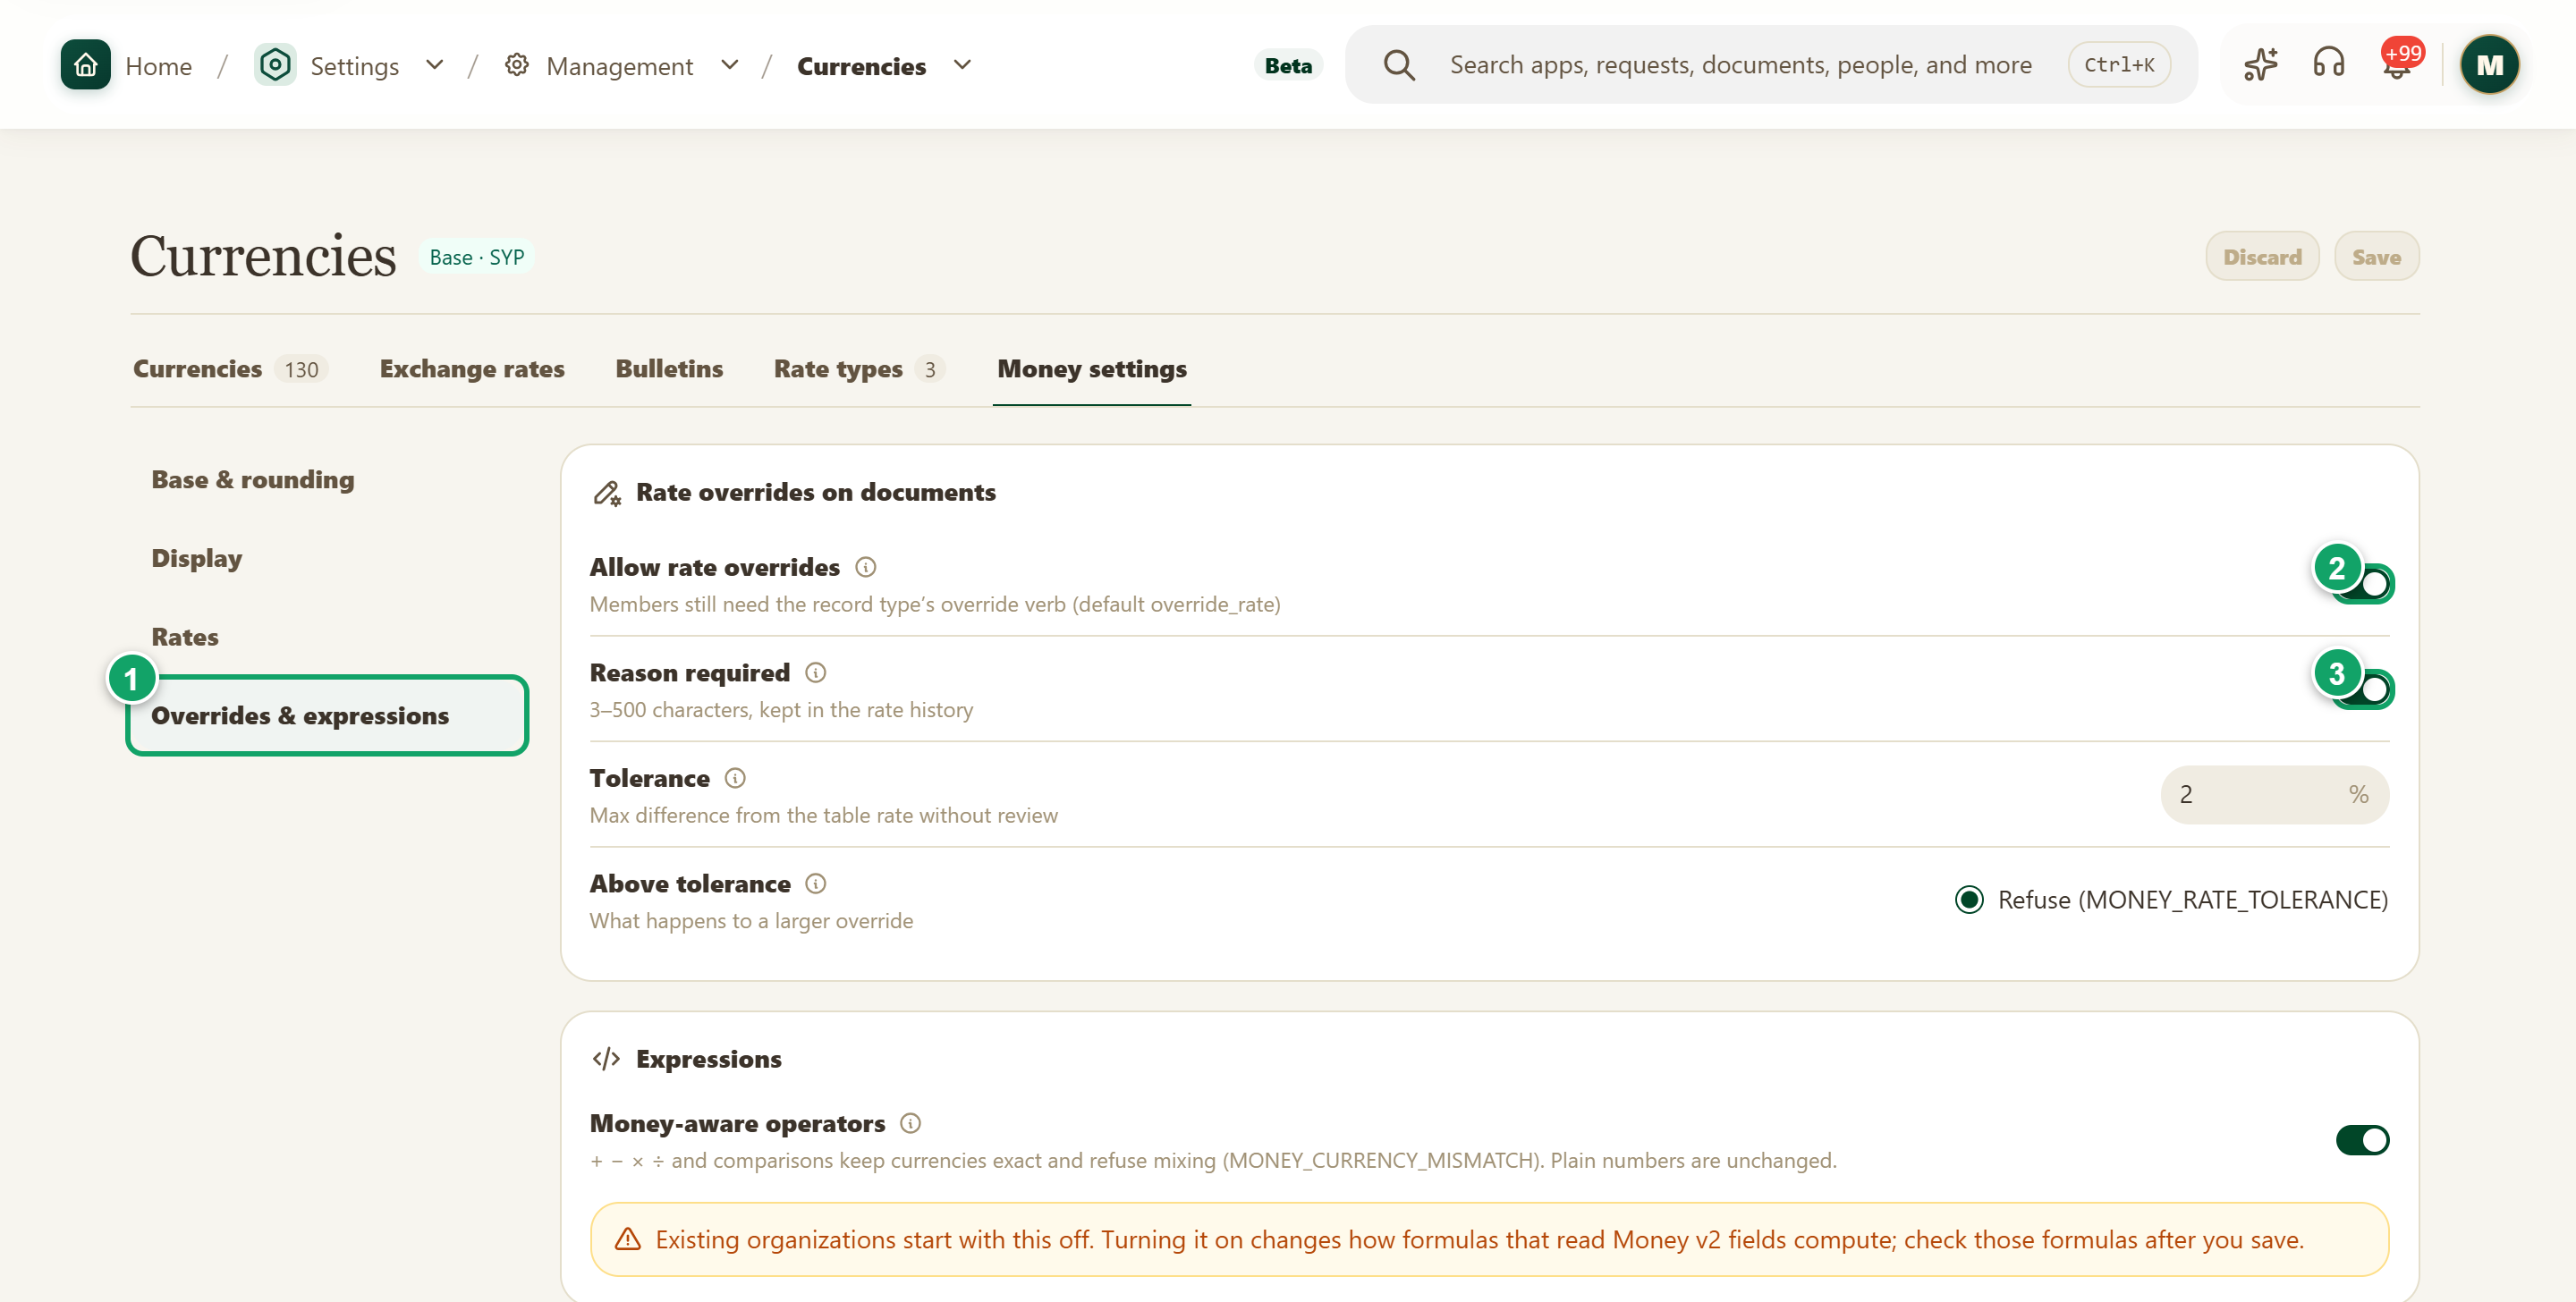
\includegraphics[width=0.95\linewidth,height=0.72\textheight,keepaspectratio]{figures/screens/ch08-currencies-settings-overrides-en.png}
\caption{Money settings: overrides and expressions}
\label{fig:settings-currencies-settings-overrides-screen}
\shotnote{This section decides whether a member may change the rate inside a document, and within what limit. Allowing it here is not enough on its own: the member also needs the override permission on the record type. ① “Overrides \& expressions”. ② “Allow rate overrides”. ③ “Reason required”: the reason stays in the rate history.}
\end{figure}

\begin{table}[H]
\centering
\caption{What can you set in Money settings?}
\label{tab:settings-currencies-money}
\begin{tabularx}{\linewidth}{R{4.2cm} Y}
\rcHeaderRow
\thh{Section} & \thh{What you can set}\\
“Base \& rounding” & The base currency, “Rounding mode”, “Rounding stage”, “Base of lines”, and “Side balance tolerance” for two-sided documents.\\
“Display” & “Digits in print”, “Group \& decimal marks”, “Negative amounts”, “Currency label” and “Equivalent on documents”.\\
“Rates” & “Default rate type”, “Rate of the day”, “Rate decimals shown”, “Use the inverse pair”, “Cross rates through”, “Outlier warning”, and what happens when a rate is missing or stale.\\
“Overrides \& expressions” & “Allow rate overrides”, “Reason required”, “Tolerance”, “Above tolerance” and “Money-aware operators”.\\
\end{tabularx}
\end{table}

\begin{enumerate}
\item Open “Settings”, then “Currencies”.
\item Open a currency’s menu and press “Edit” to activate or adjust it, or press “Add currency” if it is not listed.
\item Open “Money settings” and review the base currency before first use, because it locks afterwards.
\item Open “Exchange rates” and press “Add rate”, choose the type, currency and date, type the rate and press “Save rate”.
\item When you change “Money settings”, press “Save” at the top of the page. “Discard” returns to the saved values.
\end{enumerate}

\textbf{Check:} The currency shows “Active” in the list, and the new rate appears in “Pairs · latest rate” and in the rate column. If you mistyped a rate, do not look for an edit button: open the rate’s actions and use “Correct…”. If “Bulletins” says that no rate type takes bulletins, open “Rate types” and set “Rates come in” to “Bulletins”.

\section{Units of measurement}
\label{sec:settings-feature-units}

This page sets the units members pick from in quantity questions, shares, matrices and record fields, such as kilograms and liters. Units sit in groups. A group that converts has a “base unit” that the others convert to, so the system can add quantities typed in different units. Use the page when your organization needs a unit that is not listed. It opens for anyone with permission to list units and unit groups.

Every organization starts with built-in units. You can rename or deactivate them, but their key and conversion stay fixed. A unit that has been used keeps its conversion and cannot be deleted, so saved answers keep their meaning.

\begin{rcnote}[Example: Horizon]
Horizon receives hospitality supplies by the carton, with no known weight. So the system administrator creates a “Packs” group of type “No conversion” at ①, then adds a “Carton” unit to it at ②. Cartons are then totaled on their own and never mixed with kilograms.
\end{rcnote}

\begin{figure}[H]
\centering
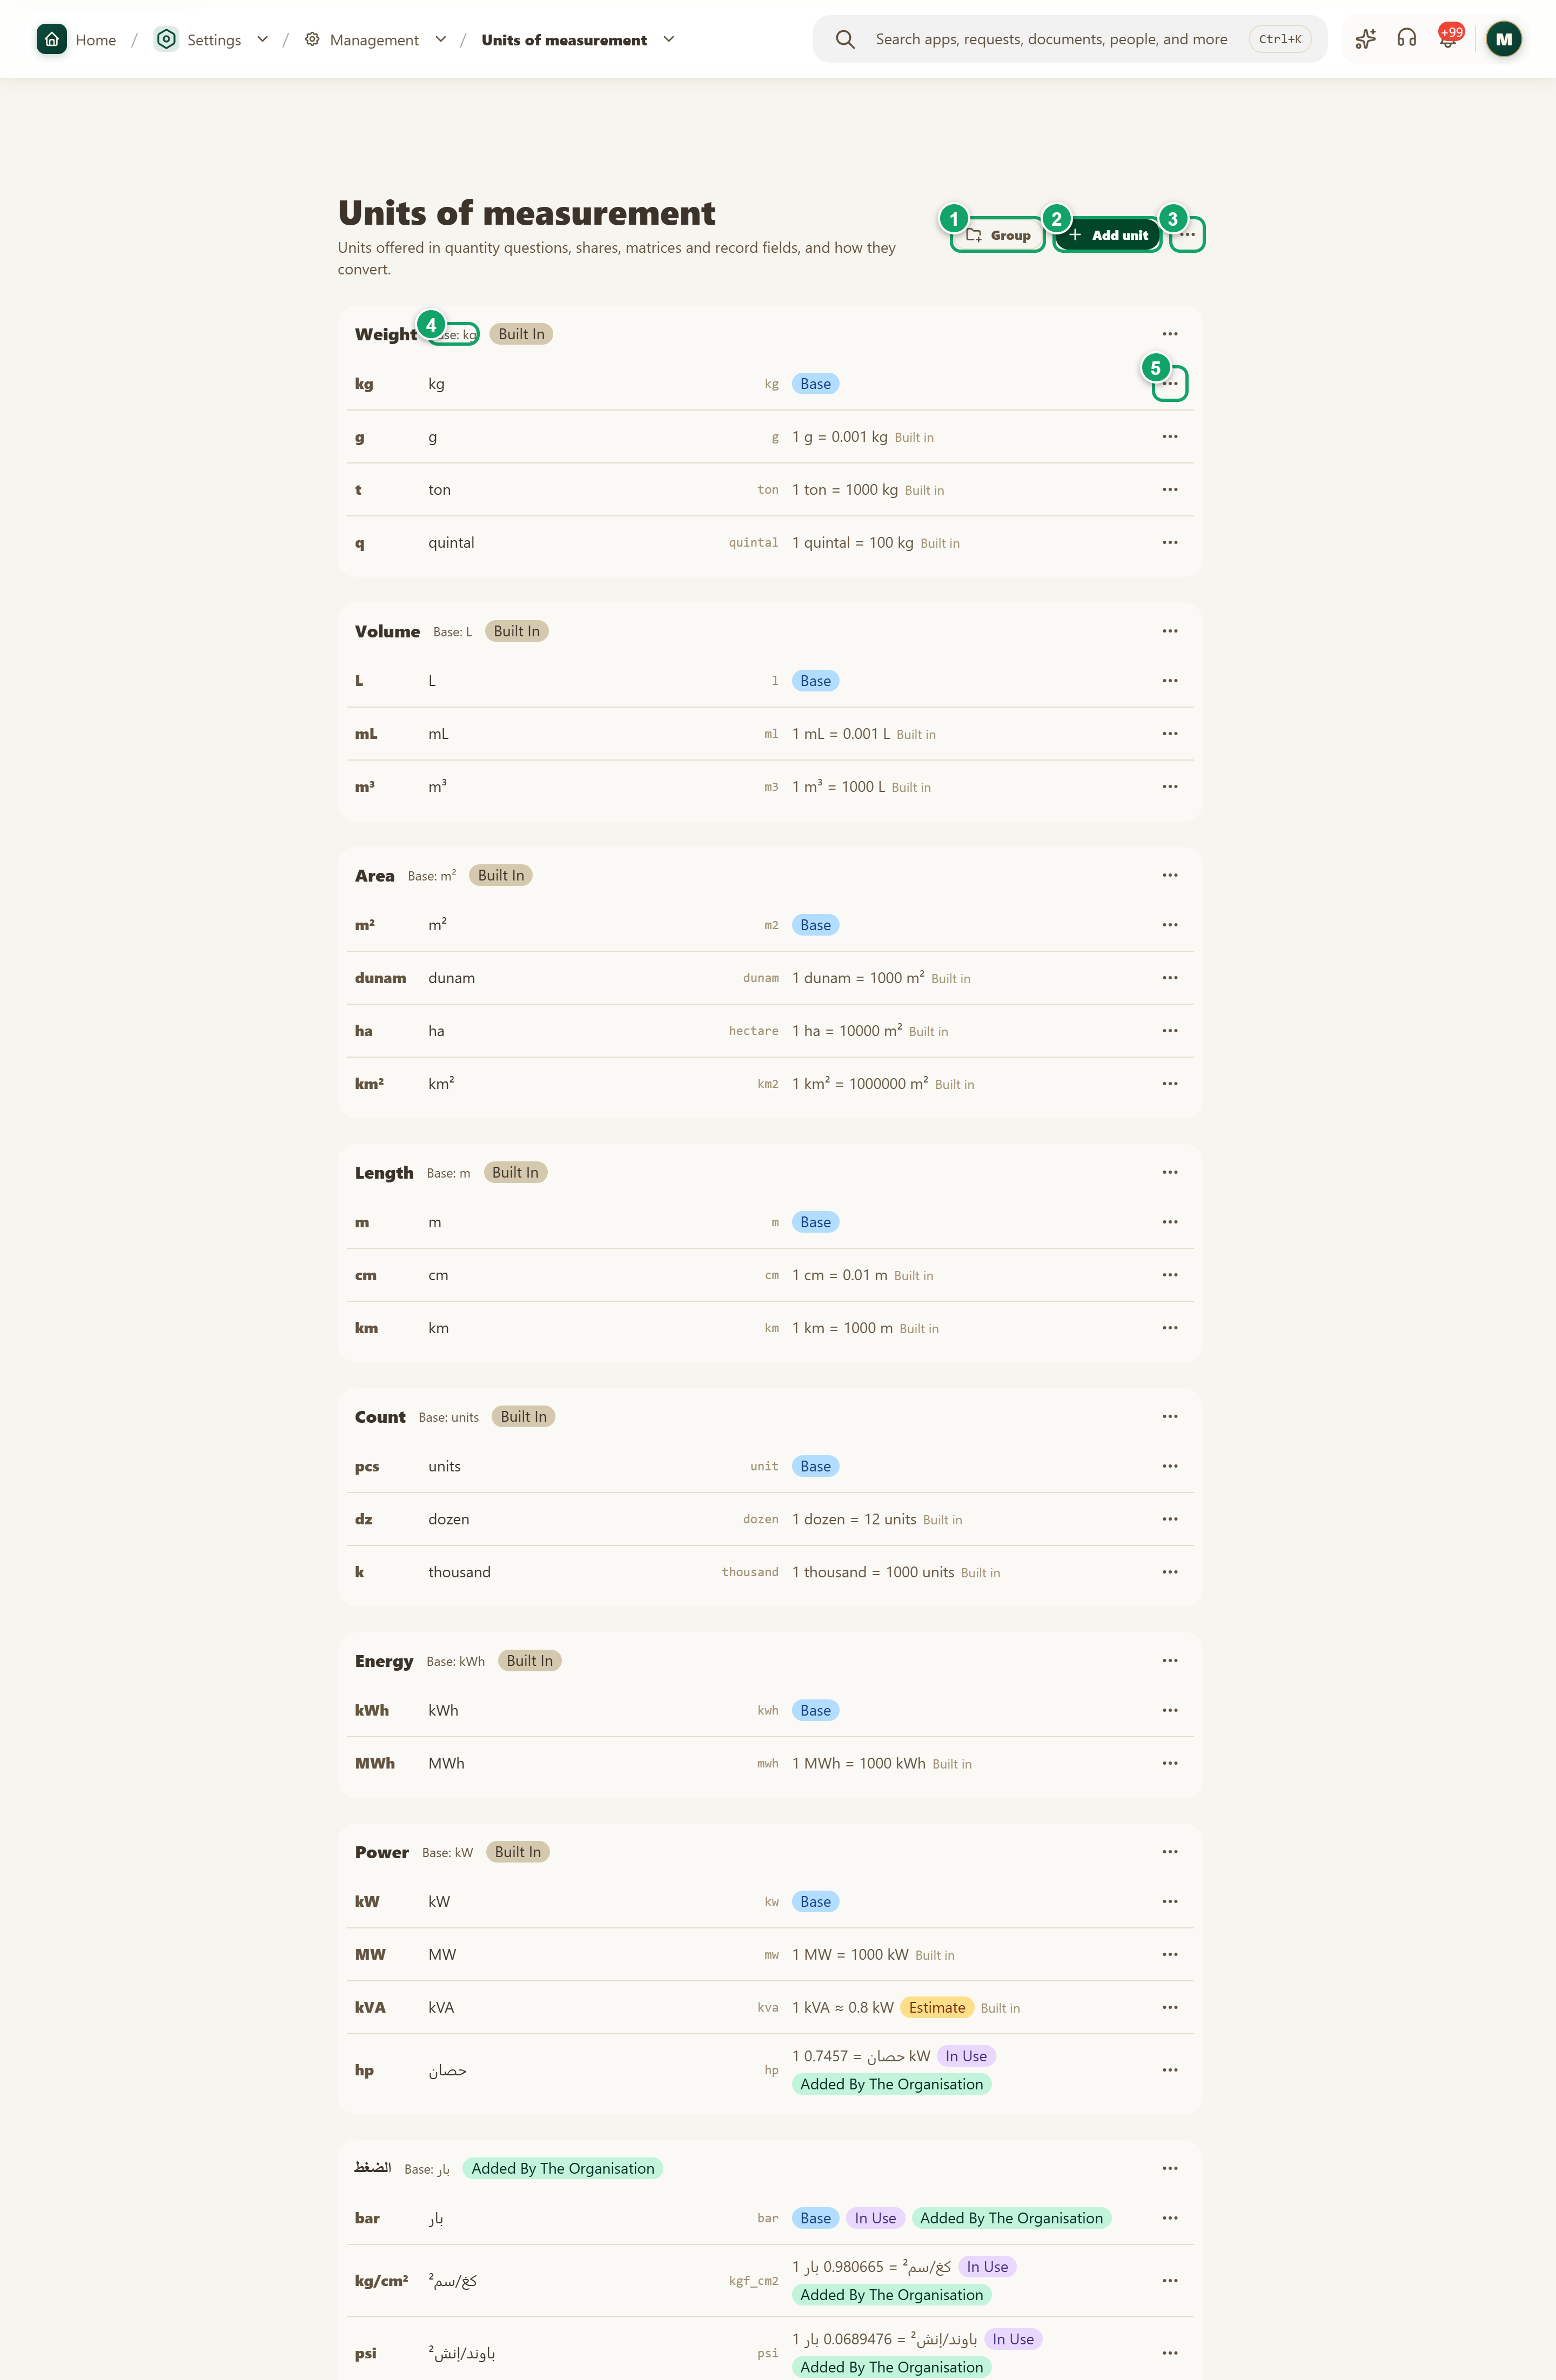
\includegraphics[width=0.95\linewidth,height=0.72\textheight,keepaspectratio]{figures/screens/ch08-units-en.png}
\caption{Unit groups}
\label{fig:settings-units-screen}
\shotnote{The page shows each group with its units and how each converts to the base. Chips show where a unit comes from and its state, such as “Built in”, “Added by the organisation” and “In use”, so you know what can change before you open it. ① “Group”. ② “Add unit”. ③ “More actions”: opens “Import units”. ④ The group’s base unit. ⑤ The unit menu: “Edit”, “Make inactive”, moving, and “Delete” when the unit can be deleted.}
\end{figure}

\begin{figure}[H]
\centering
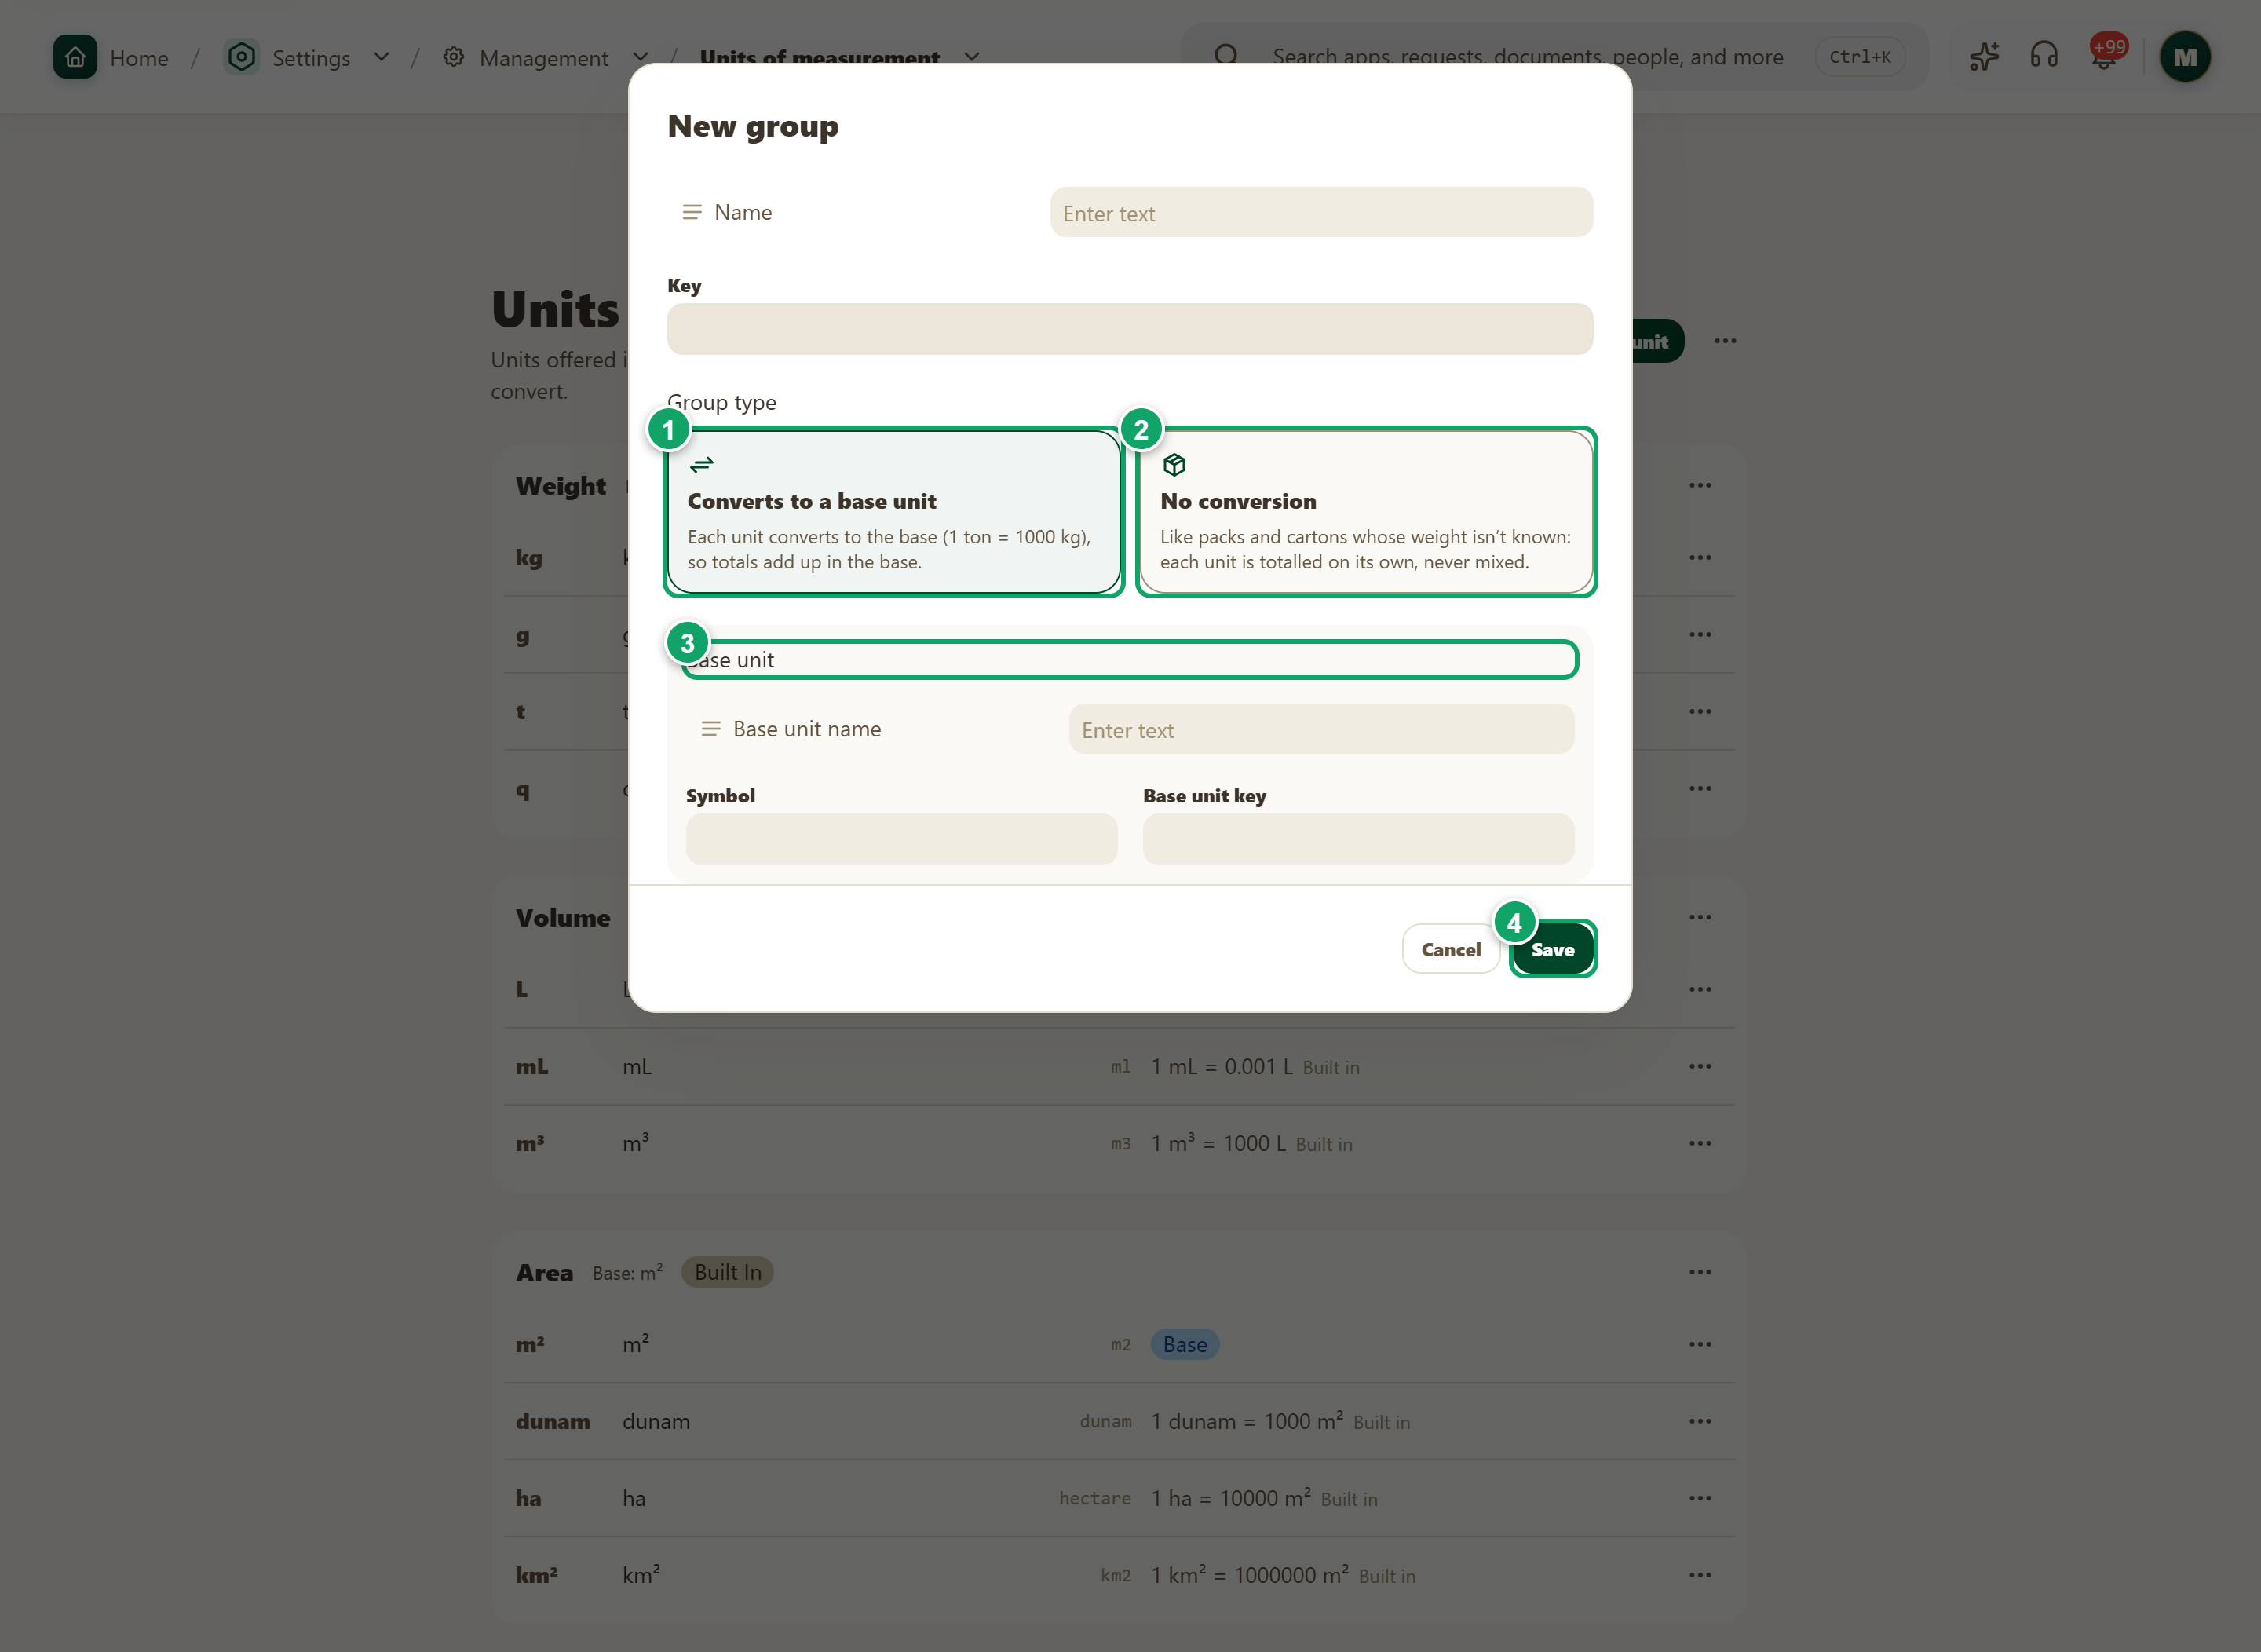
\includegraphics[width=0.95\linewidth,height=0.72\textheight,keepaspectratio]{figures/screens/ch08-units-group-en.png}
\caption{The new group window}
\label{fig:settings-units-group-screen}
\shotnote{The main decision is made when the group is created, because its type and base unit do not change afterwards. The window here is empty and was not saved. ① “Converts to a base unit”: such as 1 ton = 1000 kg. ② “No conversion”: each unit is totaled on its own. ③ “Base unit”: its name, symbol and key. ④ “Save”.}
\end{figure}

\begin{figure}[H]
\centering
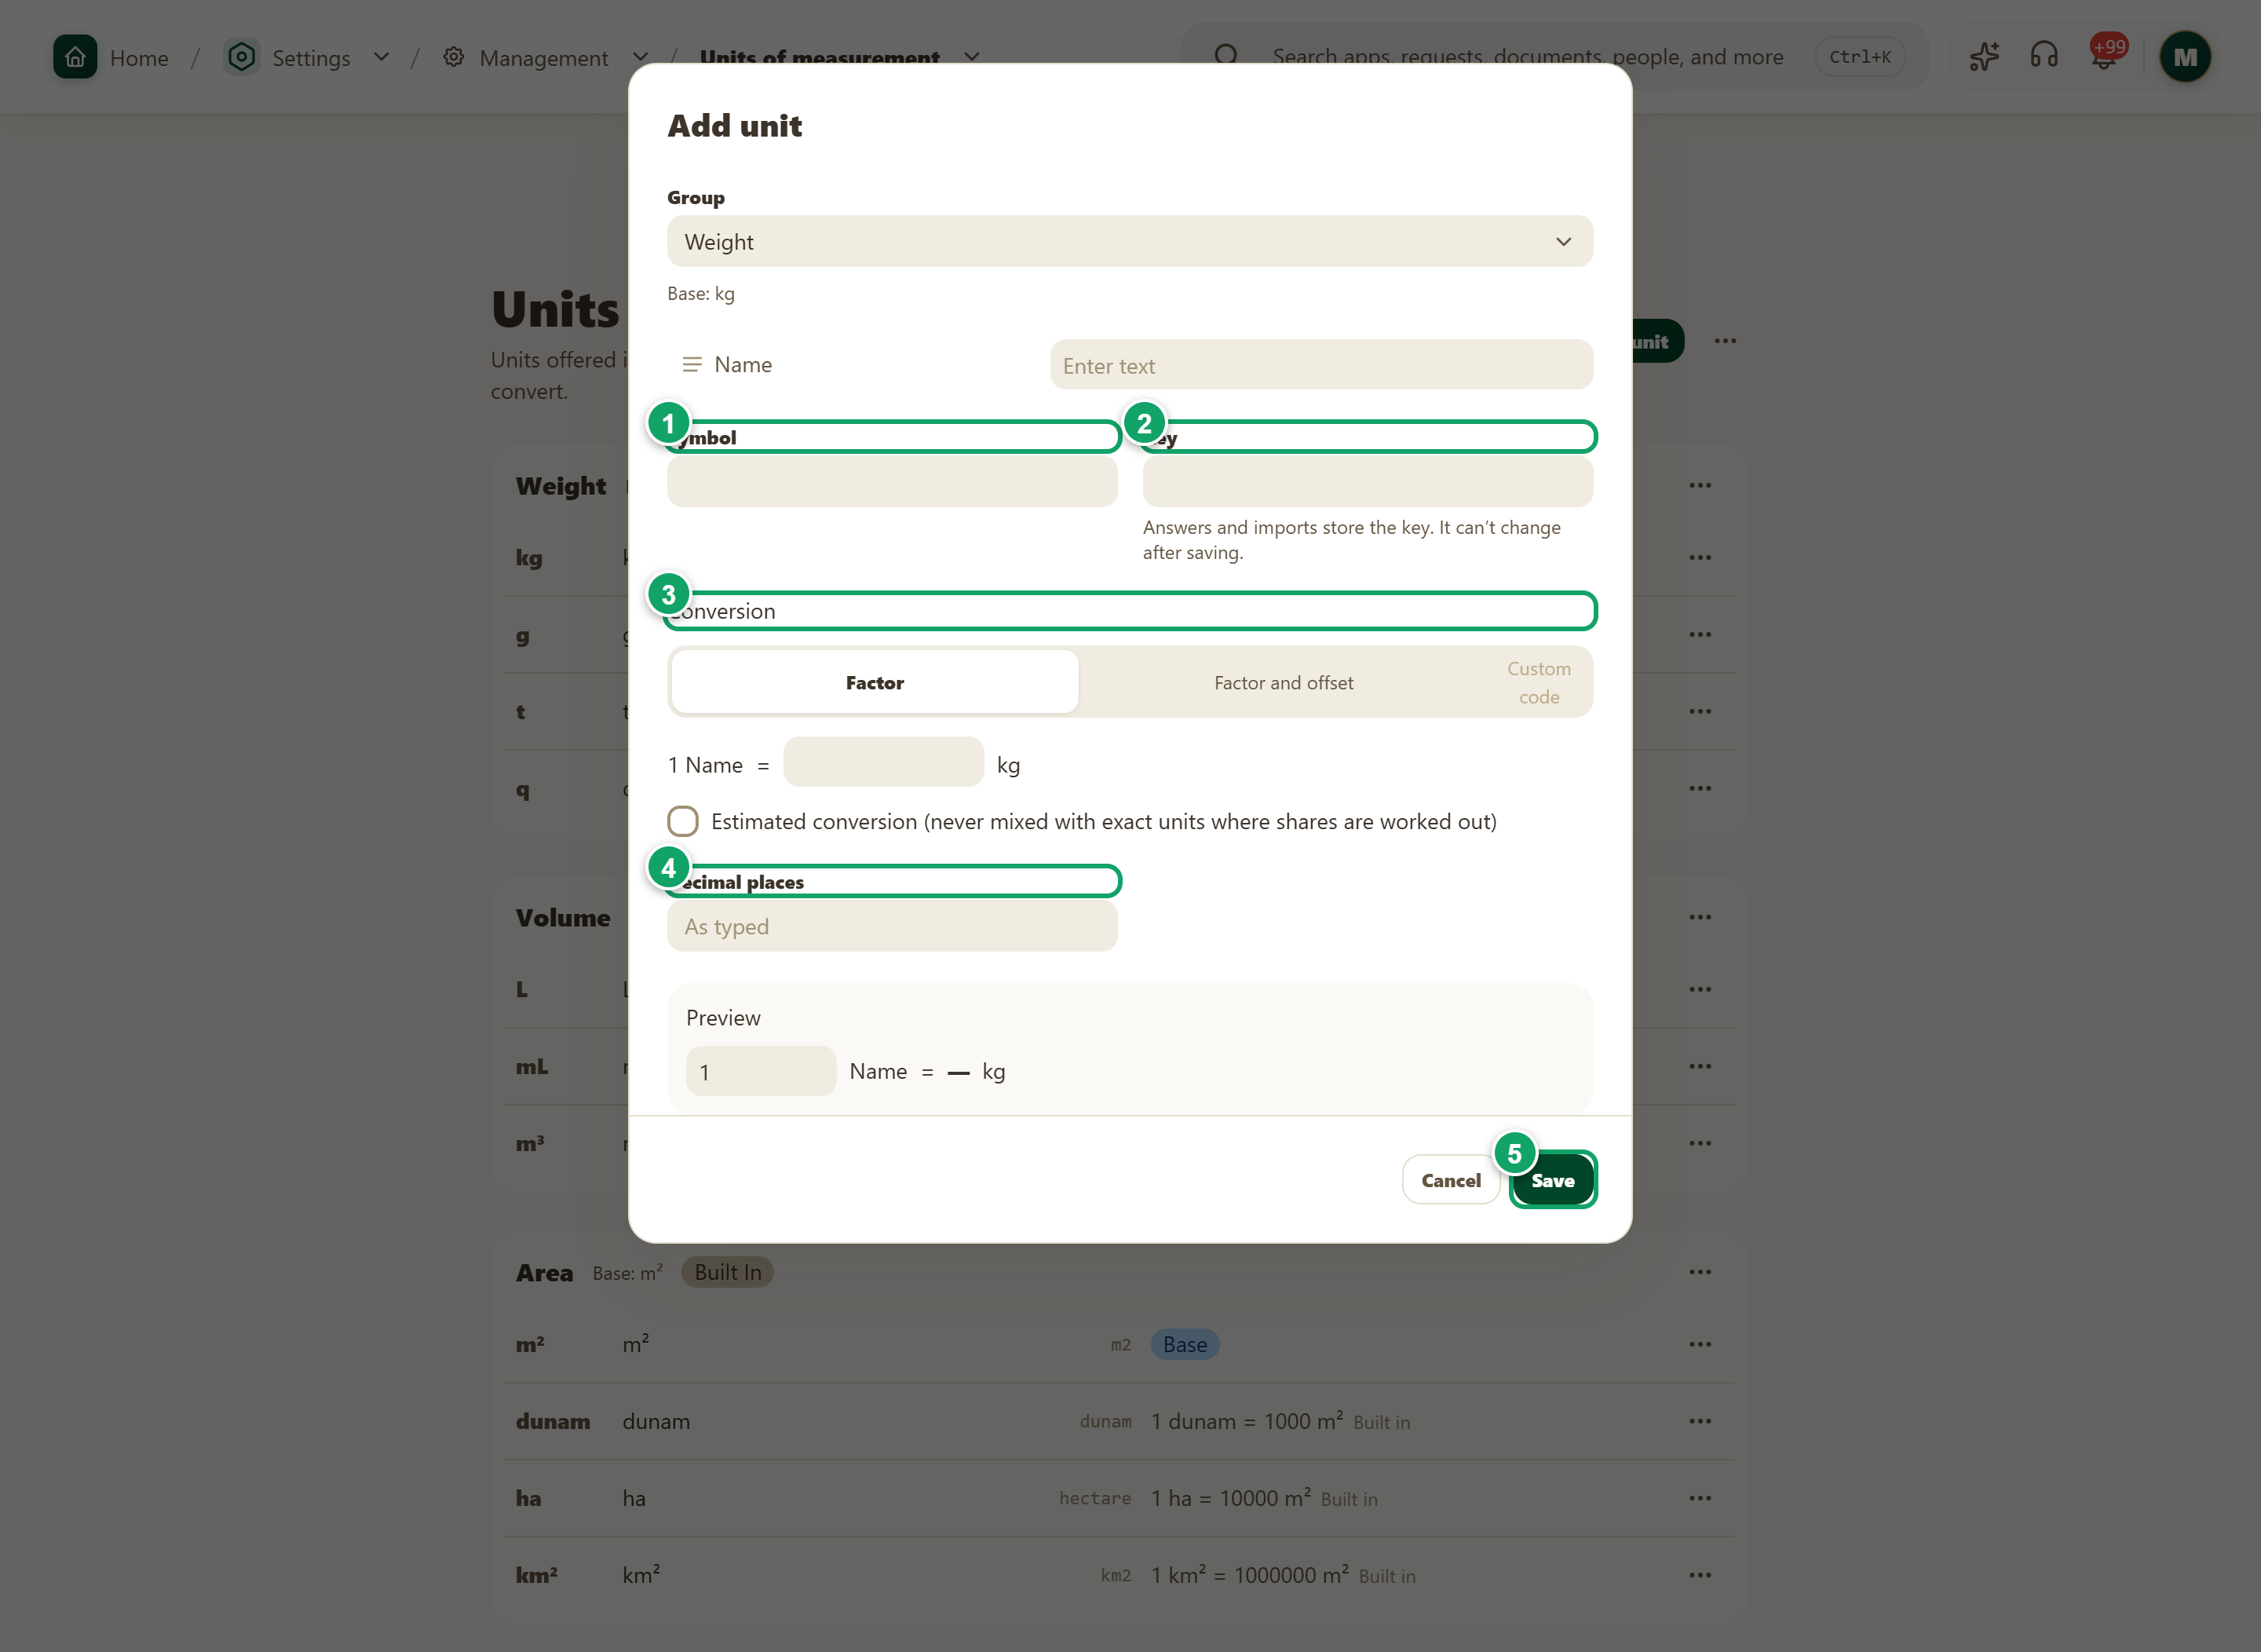
\includegraphics[width=0.95\linewidth,height=0.72\textheight,keepaspectratio]{figures/screens/ch08-units-form-en.png}
\caption{The add unit window}
\label{fig:settings-units-form-screen}
\shotnote{The window sets the unit’s name and its size against the base unit, with a preview that helps you confirm the conversion before saving. ① “Symbol”. ② “Key”: filled from the name and fixed after saving. ③ “Conversion”. ④ “Decimal places”. ⑤ “Save”.}
\end{figure}

\begin{table}[H]
\centering
\caption{What do you record for a unit and a group?}
\label{tab:settings-units-fields}
\begin{tabularx}{\linewidth}{R{4.2cm} Y}
\rcHeaderRow
\thh{Field} & \thh{Meaning}\\
“Group” & The active group the unit belongs to.\\
“Name” and “Symbol” & The name in each active language, and the short form shown beside a quantity.\\
“Key” & A fixed name that answers and imports store. It starts with a letter and uses only a–z, 0–9 and \_.\\
“Conversion” & “Factor”, such as 1 ton = 1000 kg, or “Factor and offset” for units that do not start at zero. “Custom code” is not available yet.\\
“Estimated conversion” & Set on an inexact conversion, so it is never mixed with exact units when shares are worked out.\\
“Decimal places” & A whole number from 0 to 10, or “As typed”.\\
“Words for printing” & Appears when you edit a saved unit, and sets the name’s forms when a number prints in words.\\
\end{tabularx}
\end{table}

\begin{enumerate}
\item Open “Settings”, then “Units of measurement”.
\item If you need a new group, press “Group”, enter “Name”, choose its type and press “Save”.
\item Open the group’s menu and press “Add a unit to this group”, or press “Add unit” and choose the group.
\item Enter “Name” and “Symbol”, type the factor if the group converts, then press “Save”.
\item To remove an unused unit, open its menu, press “Delete” and confirm. For a unit in use, press “Make inactive” instead.
\end{enumerate}

\textbf{Check:} The unit appears in its group with the “Added by the organisation” chip, stays there after you reload the page, and shows its conversion beside it. Reopen it with “Edit” and the “Key” is locked. Deleting a group deletes its units too, as long as none has been used.
